%%%%%%%%%%%%%%%%%%%%%%%%%%%%%%%%%%%%%%%%%
% LaTeX Template
%
% This template was downloaded from:
% http://www.LaTeXTemplates.com
%
% Version 2.x major modifications by:
% Vel (vel@latextemplates.com)
%
% Original Authors:
% Vel (vel@latextemplates.com)
% Johannes Böttcher
% Steve Gunn (http://users.ecs.soton.ac.uk/srg/softwaretools/document/templates/)
% Sunil Patel (http://www.sunilpatel.co.uk/thesis-template/)
%
% This template was modified by Muneendra Ojha to suit the needs of 
% IIIT Allahabad Students. This is a basic template consisting of all 
% requirements as approved by the institute. Please feel free to contact
% if any errors are found or updates needed.
% 
% Do not remove this preamble. Always remember to give credit where it is due.
% 
% Template license:
% CC BY-NC-SA 3.0 (http://creativecommons.org/licenses/by-nc-sa/3.0/)
%
%%%%%%%%%%%%%%%%%%%%%%%%%%%%%%%%%%%%%%%%%

%----------------------------------------------------------------------------------------
%	PACKAGES AND OTHER DOCUMENT CONFIGURATIONS
%----------------------------------------------------------------------------------------

\documentclass[
12pt, % The default document font size, options: 10pt, 11pt, 12pt
oneside, % Two side (alternating margins) for binding by default, uncomment to switch to one side
english, % ngerman for German
singlespacing, % options: singlespacing, onehalfspacing or doublespacing
%draft, % Uncomment to enable draft mode (no pictures, no links, overfull hboxes indicated)
% nolistspacing, % If the document is onehalfspacing or doublespacing, uncomment this to set spacing in lists to single
liststotoc, % Uncomment to add the list of figures/tables/etc to the table of contents
% toctotoc, % Uncomment to add the main table of contents to the table of contents
parskip, % Uncomment to add space between paragraphs
%nohyperref, % Uncomment to not load the hyperref package
headsepline, % Uncomment to get a line under the header
% chapterinoneline, % Uncomment to place the chapter title next to the number on one line
% consistentlayout, % Uncomment to change the layout of the declaration, abstract and acknowledgements pages to match the default layout
]{Thesis} % The class file specifying the document structure



\usepackage[utf8]{inputenc} % Required for inputting international characters
\usepackage[T1]{fontenc} % Output font encoding for international characters
\usepackage{mathpazo} % Use the Palatino font by default
\usepackage[backend=biber,
style=numeric,
bibencoding=utf8,
% style=authoryear, % if using style as authoryear, then cite the reference using \parencite{}
% style=reading
]{biblatex}
\DefineBibliographyStrings{english}{
  bibliography = {References},
}
\setlength\bibitemsep{15pt}
\addbibresource{references.bib} % The filename of the bibliography
\usepackage[autostyle=true]{csquotes} % Required to generate language-dependent quotes in the bibliography
\usepackage{array}% http://ctan.org/pkg/array
\usepackage{lipsum}
\usepackage{graphicx}
\usepackage{subcaption}
\usepackage{listings}
\usepackage{pdfpages}
\usepackage{float}
\usepackage{etoolbox}
\usepackage{algorithmic}
\usepackage{textcomp}
\usepackage{colortbl} % For colored table cells
\usepackage{booktabs} % For better tables
\usepackage{multirow} % For multirow cells in tables
\usepackage{url}      % For URLs
\usepackage{float}
\usepackage{subcaption}
\usepackage{threeparttable}
\usepackage{tabularx}
\usepackage{caption}
\usepackage[table]{xcolor}

% \usepackage[english]{babel}



%----------------------------------------------------------------------------------------
%	MARGIN SETTINGS
%----------------------------------------------------------------------------------------

\geometry{
	paper=a4paper, % Change to letterpaper for US letter
	inner=20mm, % Inner margin
	outer=20mm, % Outer margin
	bindingoffset=5mm, % Binding offset
	top=30mm, % Top margin
	bottom=20mm, % Bottom margin
	%showframe, % Uncomment to show how the type block is set on the page
}


%----------------------------------------------------------------------------------------
%	THESIS INFORMATION
%----------------------------------------------------------------------------------------

\thesistitle{Comparative Analysis of Lion and AdamW Optimizers for Cross-Encoder Reranking with MiniLM, GTE, and ModernBERT} % Your thesis title, this is used in the title and abstract, print it elsewhere with \ttitle
\supervisor{Dr. Muneendra Ojha} % Your supervisor's name, this is used in the title page, print it elsewhere with \supname
\examiner{} % Your examiner's name, this is not currently used anywhere in the template, print it elsewhere with \examname
\degree{Master of Technology} % Your degree name, this is used in the title page and abstract, print it elsewhere with \degreename
\firstauthor{Shahil Kumar} % Your name, this is used in the title page and abstract, print it elsewhere with \authorname
\enrollmentnumber{MML2023008} % put your university enrollment number here.
\addresses{} % Your address, this is not currently used anywhere in the template, print it elsewhere with \addressname

\subject{Information Technology} % Your subject area, this is not currently used anywhere in the template, print it elsewhere with \subjectname
\keywords{} % Keywords for your thesis, this is not currently used anywhere in the template, print it elsewhere with \keywordnames
\university{Indian Institute of Information Technology, Allahabad} % Your university's name and URL, this is used in the title page and abstract, print it elsewhere with \univname
\department{Department of Information Technology} % Your department's name and URL, this is used in the title page and abstract, print it elsewhere with \deptname
\specialization{Machine Learning and Intelligent Systems} % Your specialization name and URL, this is used in the title page, print it elsewhere with \specializationname
\faculty{Faculty Name} % Your faculty's name and URL, this is used in the title page and abstract, print it elsewhere with \facname



\AtBeginDocument{
\hypersetup{pdftitle=\ttitle} % Set the PDF's title to your title
% \hypersetup{pdfauthor=\authorname} % Set the PDF's author to your name
\hypersetup{pdfkeywords=\keywordnames} % Set the PDF's keywords to your keywords
}
\addto\captionsenglish{
  \renewcommand{\contentsname}{TABLE OF CONTENTS}
  \renewcommand{\listfigurename}{LIST OF FIGURES}
  \renewcommand{\listtablename}{LIST OF TABLES}
}
% Patch TOC title
\patchcmd{\tableofcontents}{\contentsname}{Table Of Contents}{}{}

\usepackage{hyperref}
\begin{document}
\begin{sloppypar}

%----------------------------------------------------------------------------------------
%	FRONT CONTENT
%----------------------------------------------------------------------------------------

\frontmatter% Use roman page numbering style (i, ii, iii, iv...) for the pre-content pages

\pagestyle{plain} % Default to the plain heading style until the thesis style is called for the body content
%----------------------------------------------------------------------------------------
%	TITLE PAGE
%----------------------------------------------------------------------------------------

\begin{titlepage}
\begin{center}
\begin{spacing}{1.2}

{\huge \bfseries\ttitle\par}  % Thesis title

\vspace {5mm}
\textit{A thesis submitted in partial fulfillment of the requirements\\for the award of the degree of} 

\vspace{7mm}
\textsc{\huge MASTER OF TECHNOLOGY}

\vspace {3mm}
\begin{figure}[htp]
    \centering
    
\includegraphics[scale=0.28]{./IIITA_Logo.png}
\end{figure}
% ************************************
\begin{minipage}[t]{0.5\textwidth}
    \begin{flushleft} \large
        \textit{By:-} \\%[2mm]
            \textsc{SHAHIL KUMAR} % Student Names
    \end{flushleft}
\end{minipage}
\begin{minipage}[t]{0.45\textwidth}
    \begin{flushright} \large
        \textit{Enrollment No.} \\
            \textsc{MML2023008} % Student Enrollment numbers
    \end{flushright}
\end{minipage}\\[1cm]
% *************************************

\textit{Under the Supervision of}\\[2mm]
\textsc{\Large \supname}\\% Supervisor's Name

%\textit{Under the Co-Supervision of}\\[2mm]
%\textsc{\Large Prof. Manish Goswami}\\% Supervisor's Name
\vspace{7mm}
\textit{to the}\\[2mm]
\textsc{\Large \deptname}\\ % Department

\vspace{8mm}
\begin{hindi}
    \textsc{\Large {भारतीय सूचना प्रौद्योगिकी संस्थान, इलाहाबाद}} \\
\end{hindi}
\vspace{3mm}
\textsc{\Large Indian Institute of Information Technology, Allahabad} % university

\vspace{5mm}
{\fontsize{14}{14}\selectfont \text{May , 2025}}


\end{spacing}
\end{center}
\end{titlepage}



%----------------------------------------------------------------------------------------
%	DECLARATION
%----------------------------------------------------------------------------------------
\checktoopen
\begin{figure}[htp]
    % \centering
    
\includegraphics[height=3cm,keepaspectratio]{./IIITA_Header.png}
\end{figure}
% \string\setblankpagestyle \space
\thispagestyle{empty}
\vspace{1mm}

\begin{center}
    {\large\bfseries CANDIDATE DECLARATION}
\end{center}

\begin{spacing}{1.5}
\addchaptertocentry{CANDIDATE DECLARATION}
\vspace{10 pt}
I hereby declare that work presented in the report entitled “\textbf{Comparative Analysis of Lion and AdamW Optimizers for Cross-Encoder Reranking with MiniLM, GTE, and ModernBERT}”, submitted towards the fulfillment of MASTER’S THESIS report of M.Tech at Indian Institute of Information Technology Allahabad, is an authenticated original work carried out under supervision of \textbf{Dr. Muneendra Ojha}. Due Acknowledgements have been made in the text to all other material used. the project was done in full compliance with the requirements and constraints of the prescribed curriculum. 
\end{spacing}

\begin{spacing}{2.0}
\begin{flushright}
    \begin{minipage}{0.5\textwidth}
        \flushright \vspace{60 pt}
        \underline{\hspace{6cm}} \\
        \makebox[6cm]{\textbf{Shahil Kumar - MML2023008}} \\[80pt]
    \end{minipage}
\end{flushright}
\end{spacing}
\newpage

%----------------------------------------------------------------------------------------
%	CERTIFICATE
%----------------------------------------------------------------------------------------
\checktoopen
\begin{figure}[htp]
    % \centering
    
\includegraphics[height=3cm,keepaspectratio]{./IIITA_Header.png}
\end{figure}
% \string\setblankpagestyle \space
\thispagestyle{empty}
\vspace*{.06\textheight}

\begin{spacing}{1.5}
\addchaptertocentry{CERTIFICATE FROM SUPERVISORS}
\begin{center}
    {\centering\large\bfseries CERTIFICATE FROM SUPERVISORS\par\vspace{10pt}}
\end{center}

\noindent It is certified that the work contained in the thesis titled \enquote{\textbf{Comparative Analysis of Lion and AdamW
Optimizers for Cross-Encoder Reranking with MiniLM, GTE, and ModernBERT}} by \textbf{Shahil kumar} has been carried out under supervision of \textbf{Dr. Muneendra Ojha} and that this work has not been submitted elsewhere for a degree.

\vspace{3.5cm}

\hfill\begin{minipage}{7.5cm}
    \begin{spacing}{1.2}
        \par
        \rule{\textwidth}{0.2pt}\\
        {Dr. Muneendra Ojha} \par
        {\deptname}  \par
        IIIT Allahabad \par
    \end{spacing}
\end{minipage}


\end{spacing}
% \end{certificate}
\cleardoublepage

\begin{figure}[htp]
    % \centering
    
\includegraphics[height=3cm,keepaspectratio]{./IIITA_Header.png}
\end{figure}
% \string\setblankpagestyle \space
\thispagestyle{empty}
\vspace*{.06\textheight}

\begin{spacing}{1.5}
\addchaptertocentry{CERIFICATE OF APPROVAL}
\begin{center}
    {\centering\large\bfseries CERTIFICATE OF APPROVAL \par\vspace{10pt}}
\end{center}

 This thesis entitled \textbf{Comparative Analysis of Lion and AdamW Optimizers for Cross-Encoder Reranking with MiniLM, GTE, and ModernBERT}  by \textbf{Shahil Kumar} (MML2023008) is approved for the degree of Master's thesis at IIIT Allahabad  It is understood that by this approval, the undersigned does not necessarily endorse or approve any statement made, opinion expressed, or conclusion drawn therein but approves the thesis only for the purpose for which it is submitted."\\[40 pt]

 Signature and name of the committee members (on final examination and approval of the thesis): \\[10 pt]
 \begin{flushleft}
     \begin{enumerate}
         \item Dr. Muneendra Ojha \\[25pt]
         \item Dr. Kavindra Kandpal\\[25 pt]
         \item Dr. Anand Kumar Tiwari \\[25 pt]

     \end{enumerate}
 \end{flushleft}
 \vspace{20 pt}
 \begin{flushright}
     \begin{minipage}{0.5\textwidth}
        \flushright \vspace{60 pt}
        \underline{\hspace{6cm}} \\
        \makebox[6cm]{\textbf{Dean(A\&R)}} \\[80pt]
    \end{minipage}
 \end{flushright}
\end{spacing} 

\newpage
\addchaptertocentry{PLAGIARISM REPORT}
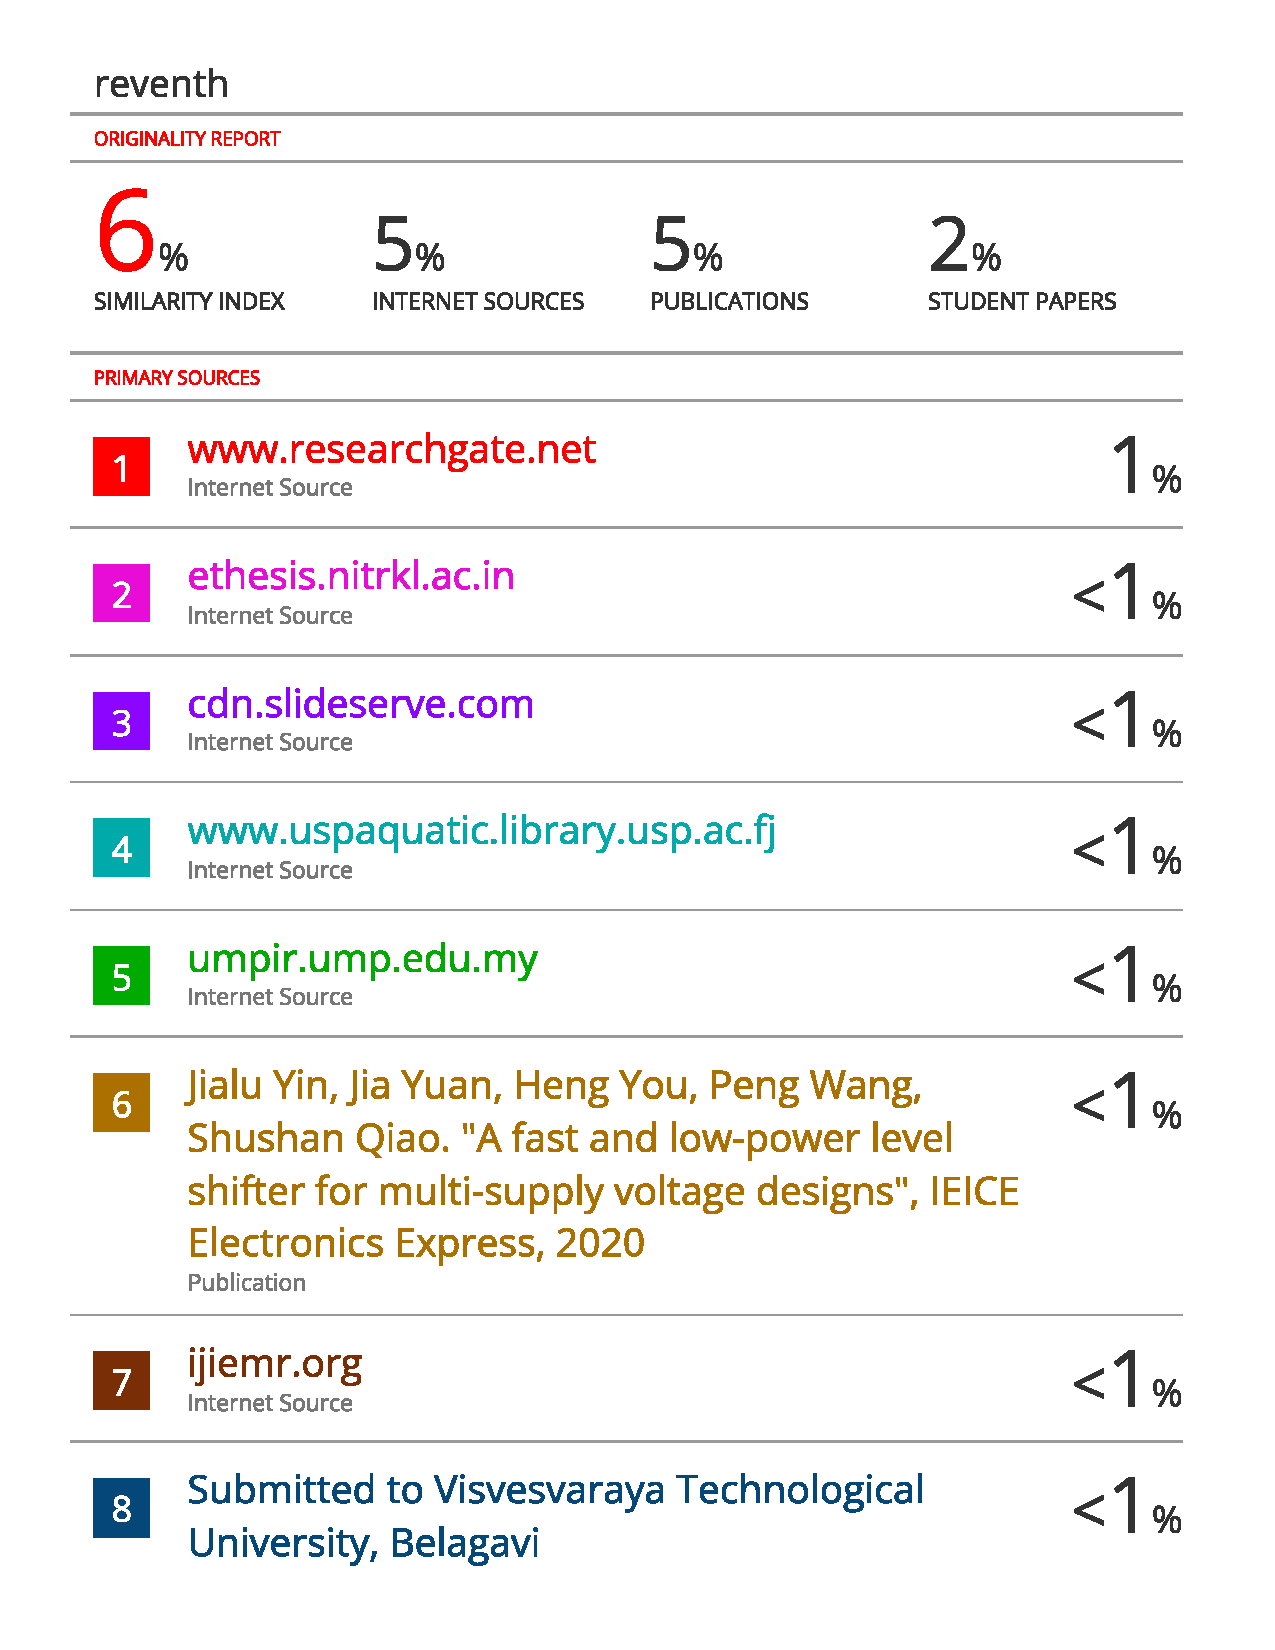
\includepdf[pages=-]{plagrevanth.pdf}
\newpage
\begin{figure}[htp]
    % \centering
    
\includegraphics[height=3cm,keepaspectratio]{./IIITA_Header.png}
\end{figure}
% \string\setblankpagestyle \space
\thispagestyle{empty}
\vspace{1mm}

\begin{center}
    {\large\bfseries ACKNOWLEDGEMENT}
\end{center}

\begin{spacing}{1.5}
\addchaptertocentry{ACKNOWLEDGEMENT}
I am thankful to my project supervisor, \textbf{Dr. Muneendra Ojha} for the guidance, support, and invaluable feedback throughout the research process. Their expertise, encouragement, and patience have been instrumental in the completion of this thesis.\\[10pt] 
 I am grateful to Dr. K.P. Singh, Head of the Department of Information Technology, and also my panel members Dr Kavindra Kandpal and Prof. Anand Kumar for their guidance and support.\\[10pt]
 I would also like to thank the Indian Institute of Information Technology, Allahabad for providing the necessary resources and facilities to conduct this research. I am deeply grateful to the participants who generously shared their time and personal information to make this study possible. \\[30 pt]
\end{spacing}

\begin{spacing}{2.0}
\begin{flushright}
    \begin{minipage}{0.5\textwidth}
        \flushright \vspace{60 pt}
        \underline{\hspace{6cm}} \\
        \makebox[6cm]{\textbf{Shahil Kumar - MML2023008}} \\[80pt]
    \end{minipage}
\end{flushright}
\end{spacing}
\newpage


\begin{center}
    {\large\bfseries ABSTRACT}
\end{center}
\begin{spacing}{1.5}
\addchaptertocentry{ABSTRACT} % Add the abstract to the table of contents
     Modern information retrieval systems often employ a two-stage pipeline consisting of an efficient initial retrieval stage followed by a more computationally intensive reranking stage. Cross-encoder models have demonstrated state-of-the-art effectiveness for the reranking task due to their ability to perform deep, contextualized analysis of query-document pairs. The choice of optimizer during the fine-tuning phase can significantly impact the final performance and training efficiency of these models. This paper investigates the impact of using the recently proposed Lion optimizer compared to the widely used AdamW optimizer for fine-tuning cross-encoder rerankers. We fine-tune three distinct transformer models, `microsoft/MiniLM-L12-H384-uncased`, `Alibaba-NLP/gte-multilingual-base`, and `answerdotai/ModernBERT-base`, on the MS MARCO passage ranking dataset using both optimizers. Notably, GTE and ModernBERT support longer context lengths (8192 tokens). The effectiveness of the resulting models is evaluated on the TREC 2019 Deep Learning Track passage ranking task and the MS MARCO development set (for MRR@10). Our experiments, facilitated by the Modal cloud computing platform for GPU resource management, show comparative results across three training epochs. ModernBERT trained with Lion achieved the highest NDCG@10 (0.7225) and MAP (0.5121) on TREC DL 2019, while MiniLM trained with Lion tied with ModernBERT with Lion on MRR@10 (0.5988) on MS MARCO dev. We analyze the performance trends based on standard IR metrics, providing insights into the relative effectiveness of Lion versus AdamW for different model architectures and training configurations in the context of passage reranking.
\end{spacing}


\newpage


%----------------------------------------------------------------------------------------
%	LIST OF CONTENTS/FIGURES/TABLES PAGES
%----------------------------------------------------------------------------------------
\addchaptertocentry{Table of Contents}
\tableofcontents % Prints the main table of contents
\listoffigures
\listoftables

%----------------------------------------------------------------------------------------
%	ABBREVIATIONS
%----------------------------------------------------------------------------------------
% \chapter*{List of Abbreviations}
% \addcontentsline{toc}{chapter}{List of Abbreviations}
% \begin{tabular}{@{}ll}
%     Machine Learning Models\\
%     $E_{m}$ & Energy level\\
%     $S_{m}$ & MMSE estimation \\
%     SNR\\
%     Ambient Back scattering Communication \\
%     SVM, RF, DT, XGB \\
%     BER and reflection Coefficient \\
%     Tag decode \\
%     % Add more as needed
% \end{tabular}

%----------------------------------------------------------------------------------------
%	PHYSICAL CONSTANTS/OTHER DEFINITIONS
%----------------------------------------------------------------------------------------

% \begin{constants}{lr@{${}={}$}l} % The list of physical constants is a three column table

% % The \SI{}{} command is provided by the siunitx package, see its documentation for instructions on how to use it

% Speed of Light & $c_{0}$ & \SI{2.99792458e8}{\meter\per\second} (exact)\\
% Constant Name & $Symbol$ & $Constant Value$ with units\\

% \end{constants}

%----------------------------------------------------------------------------------------
%	SYMBOLS
%----------------------------------------------------------------------------------------

% \begin{symbols}{lll} % Include a list of Symbols (a three column table)

% $a$ & distance & \si{\meter} \\
% $P$ & power & \si{\watt} (\si{\joule\per\second}) \\
% %Symbol & Name & Unit \\

% \addlinespace % Gap to separate the Roman symbols from the Greek

% $\omega$ & angular frequency & \si{\radian} \\

% \end{symbols}

%----------------------------------------------------------------------------------------
%	DEDICATION
%----------------------------------------------------------------------------------------

%----------------------------------------------------------------------------------------
%	THESIS CONTENT - CHAPTERS
%----------------------------------------------------------------------------------------

\mainmatter % Begin numeric (1,2,3...) page numbering

\pagestyle{thesis} % Return the page headers back to the "thesis" style
\begin{spacing}{2}
    

% Include the chapters of the thesis as separate files from the Chapters folder
% Uncomment the lines as you write the chapters

% Chapter 1

\chapter{Introduction} % Main chapter title

\label{Chapter1} % For referencing the chapter elsewhere, use \ref{Chapter1} 

%----------------------------------------------------------------------------------------

% Define some commands to keep the formatting separated from the content 
\newcommand{\keyword}[1]{\textbf{#1}}
\newcommand{\tabhead}[1]{\textbf{#1}}
\newcommand{\code}[1]{\texttt{#1}}
\newcommand{\file}[1]{\texttt{\bfseries#1}}
\newcommand{\option}[1]{\texttt{\itshape#1}}



Information Retrieval (IR) systems enable users to find relevant information from vast document collections. Modern IR systems employ a two-stage pipeline: efficient initial retrieval (BM25 \cite{robertson2009probabilistic} or dense vector retrieval \cite{karpukhin2020dense}) followed by sophisticated reranking for precision optimization.

Cross-encoder models represent the state-of-the-art for reranking \cite{nogueira2020passagererankingbert,Nogueira2020Document} due to their ability to model deep query-document interactions. Unlike bi-encoders that process queries and documents independently, cross-encoders simultaneously analyze query-document pairs, enabling rich token-level interactions for accurate relevance estimation.

The effectiveness of cross-encoder models depends heavily on optimization strategies during fine-tuning. While AdamW \cite{loshchilov2019decoupled} has been the standard choice for transformer training, recent developments in optimization algorithms, particularly the Lion optimizer \cite{chen2023symbolic}, have shown promising results across various domains, motivating investigation into their applicability for information retrieval tasks.

%----------------------------------------------------------------------------------------

\section{Cross-Encoder Models for Information Retrieval}

Cross-encoders process query-document pairs by concatenating them with special tokens ([CLS] query [SEP] document [SEP]) and feeding the combined sequence through a transformer architecture \cite{devlin2019bert}. The [CLS] token representation predicts relevance scores through a linear layer with sigmoid activation.

Modern implementations leverage various transformer architectures with distinct characteristics:
\begin{itemize}
\item \textbf{MiniLM-L12-H384}: Distilled BERT variant optimized for efficiency \cite{wang2020minilm} (512 tokens context)
\item \textbf{GTE-multilingual-base}: Extended context model (8192 tokens) with multilingual training \cite{li2023towards}
\item \textbf{ModernBERT-base}: State-of-the-art architecture with RoPE \cite{su2023roformerenhancedtransformerrotary}, Flash Attention \cite{dao2022flashattentionfastmemoryefficientexact}, and GeGLU \cite{shazeer2020gluvariantsimprovetransformer} \cite{modernbert}
\end{itemize}

\begin{figure}[!htp]
    \centering
    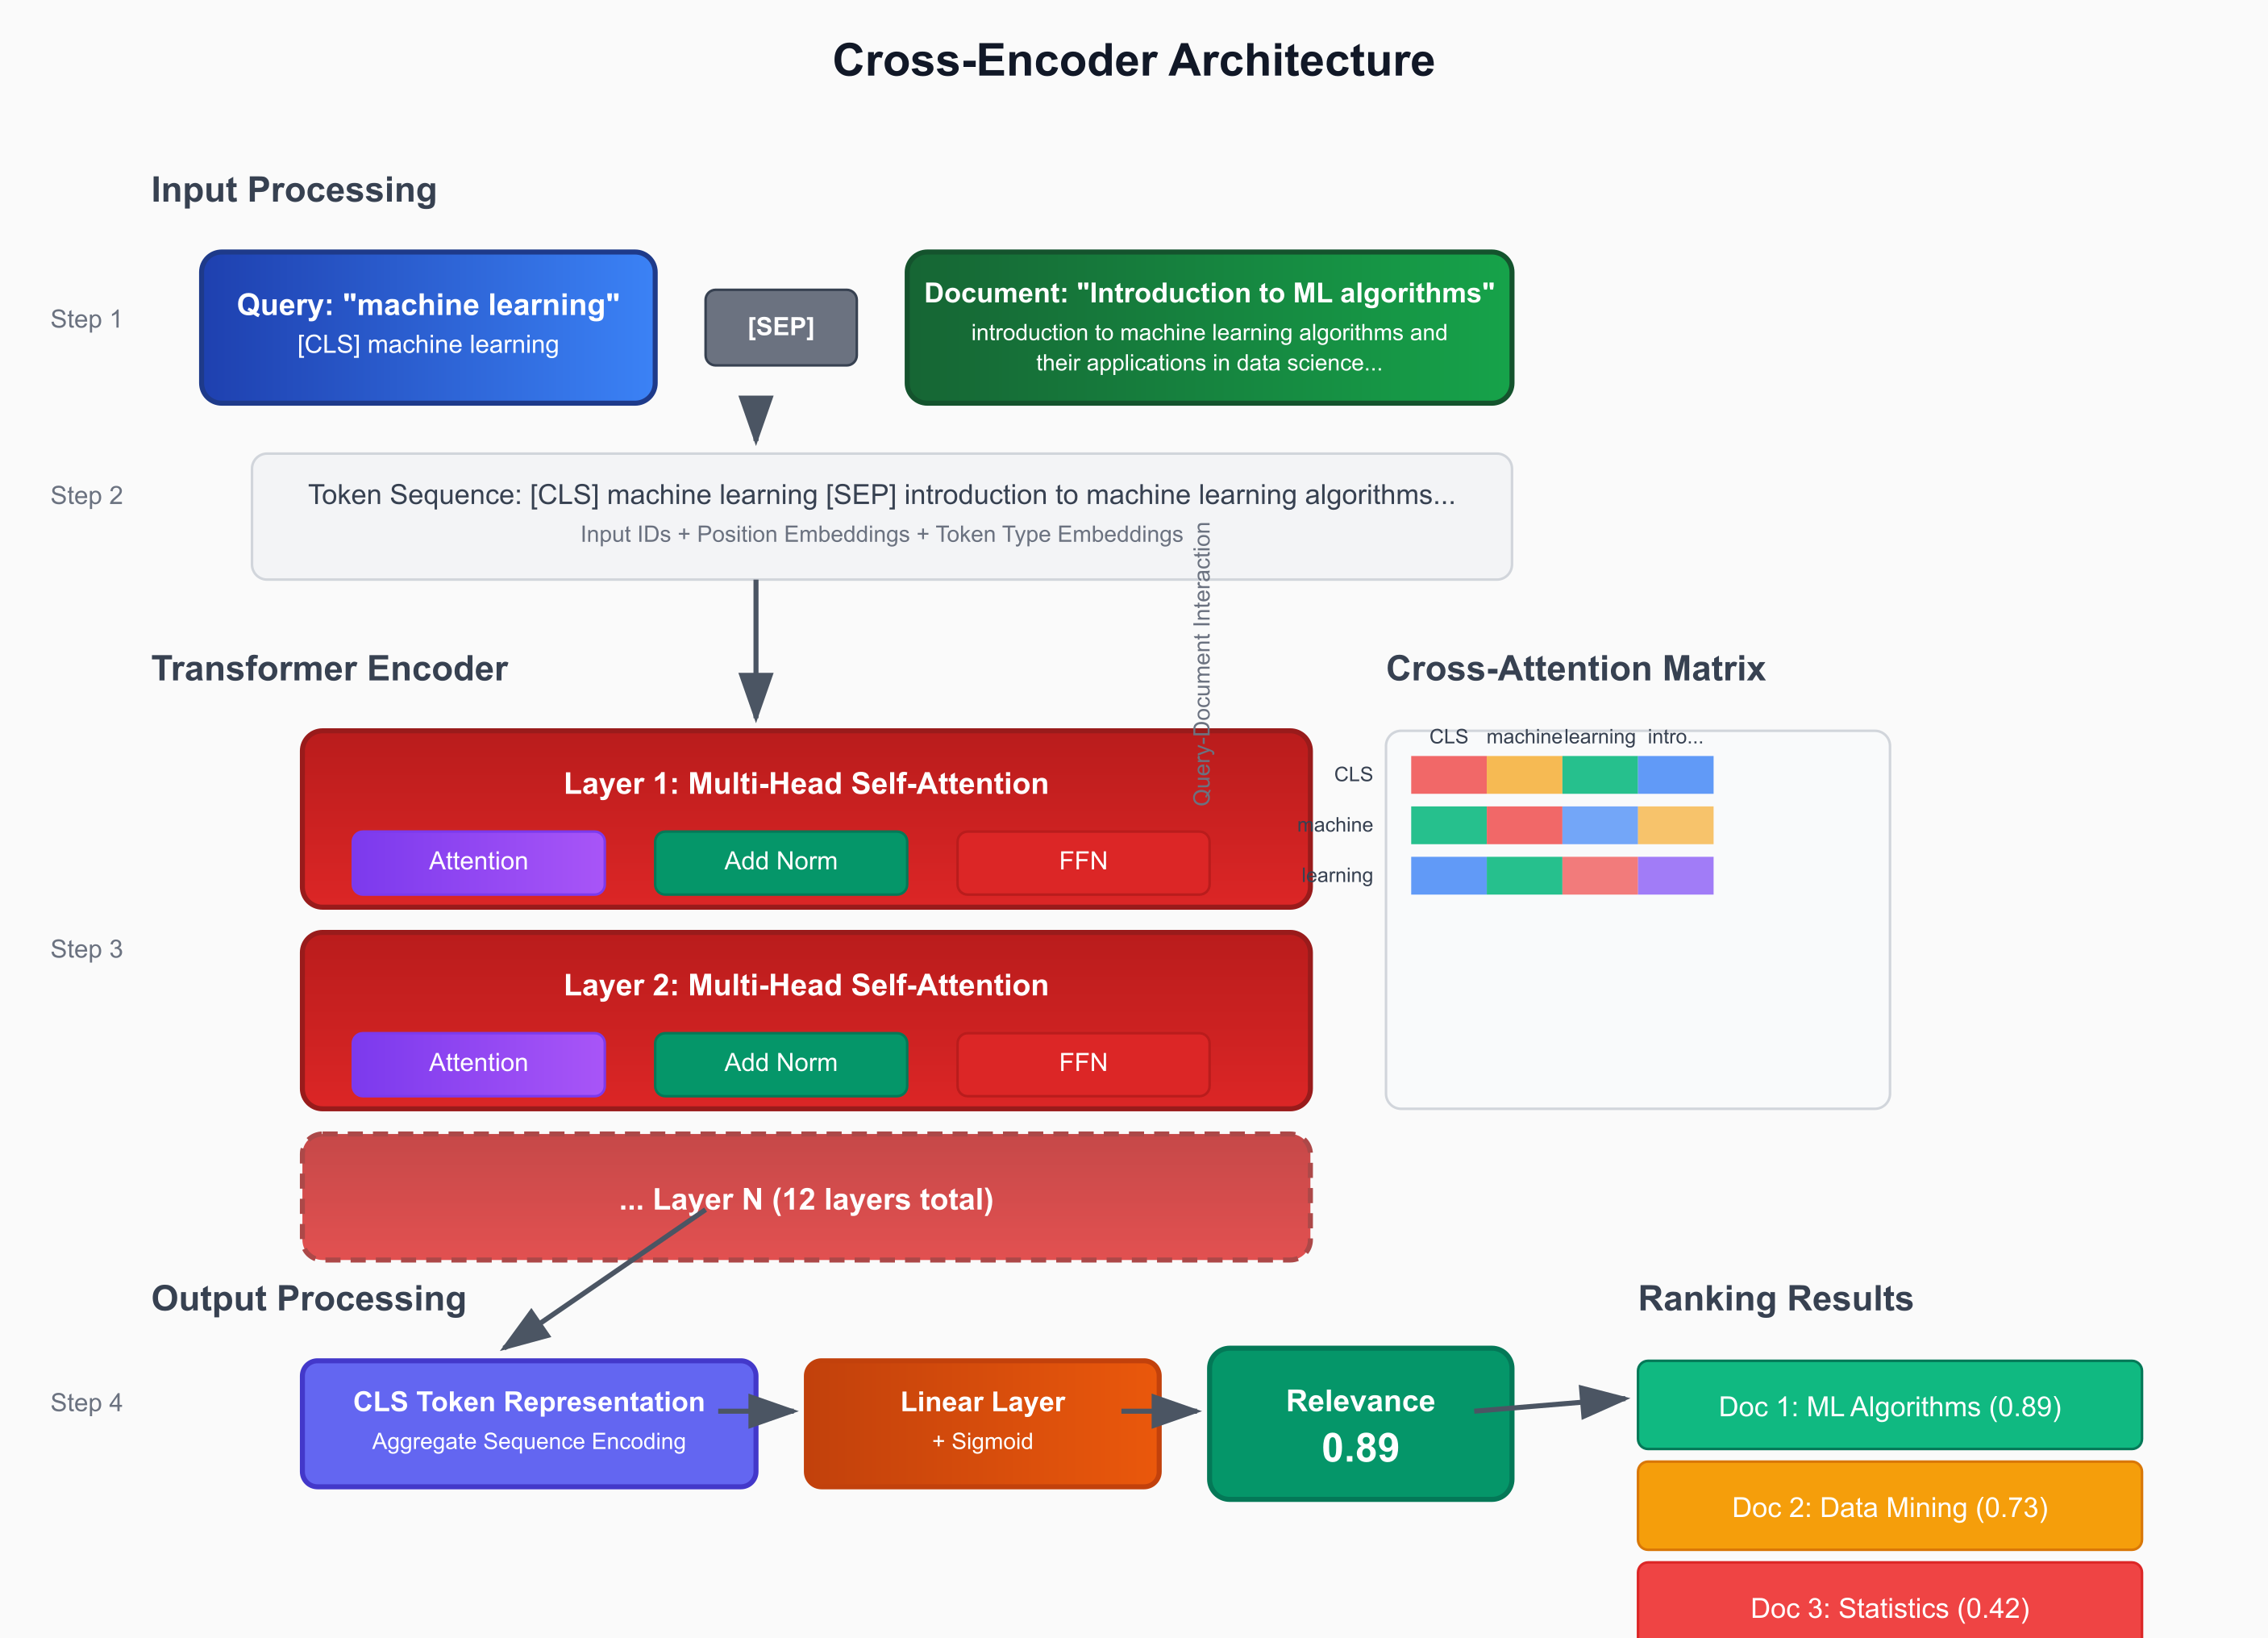
\includegraphics[width=\textwidth, keepaspectratio]{Figures/cross_encoder_archi.png}
    \caption{Cross-Encoder Architecture for Query-Document Reranking.}
    \label{fig:Cross-Encoder-Architecture}
\end{figure}

\section{Optimization Strategies}

Cross-encoder effectiveness depends on optimization strategies during fine-tuning. While AdamW \cite{loshchilov2019decoupled} has been the standard choice, the Lion optimizer \cite{chen2023symbolic} presents a novel approach using sign-based momentum: \texttt{update = sign(momentum) * learning\_rate}. This simplification offers potential memory efficiency and different convergence characteristics compared to traditional adaptive methods.

\section{Research Objectives}

This research conducts a comprehensive comparative analysis of Lion and AdamW optimizers for cross-encoder models in information retrieval. Our primary objectives are:

\begin{enumerate}
    \item \textbf{Systematic Evaluation}: Compare Lion and AdamW across three transformer architectures (MiniLM, GTE, ModernBERT)
    \item \textbf{Comprehensive Benchmarking}: Evaluate performance using standard IR metrics on TREC DL 2019 and MS MARCO
    \item \textbf{Training Dynamics Analysis}: Investigate convergence patterns and stability across training epochs
    \item \textbf{Practical Guidelines}: Provide evidence-based recommendations for optimizer selection
\end{enumerate}

\subsection{Expected Contributions}
\begin{itemize}
\item Empirical evidence comparing Lion and AdamW optimizers across multiple architectures
\item Optimization guidelines for cross-encoder training in information retrieval
\item Analysis of training efficiency and convergence characteristics
\end{itemize}

\section{Methodology Overview}

We employ systematic experimentation across three transformer architectures representing different performance-efficiency trade-offs: MiniLM (efficient baseline), GTE (extended context), and ModernBERT (state-of-the-art). Experiments utilize standardized datasets (MS MARCO \cite{DBLP:journals/corr/NguyenRSGTMD16} for training, TREC DL 2019 \cite{craswell2020overview} for evaluation) with cloud infrastructure (Modal platform \cite{modal_labs}, NVIDIA A100-80GB GPUs) ensuring reproducible results. Comprehensive tracking through Weights \& Biases \cite{wandb2020} enables detailed training dynamics analysis.

\section{Thesis Organization}

This thesis systematically presents research methodology, experimental results, and implications:
\textbf{Chapter 2}: Literature review on cross-encoder architectures and optimization algorithms
\textbf{Chapter 3}: Research gaps and proposed comparative evaluation approach  
\textbf{Chapter 4}: Experimental methodology and implementation details
\textbf{Chapter 5}: Comprehensive results with training dynamics and statistical analysis
\textbf{Chapter 6}: Key findings, implications, and future research directions

The thesis contributes empirical insights into optimizer selection for cross-encoder architectures with implications for search engines, question-answering systems, and information retrieval applications where ranking quality is paramount.

\chapter{Literature Review}
\label{Chapter2}

This chapter reviews key literature on cross-encoder models, optimization algorithms, and evaluation methodologies for information retrieval.

\section{Neural Information Retrieval Evolution}

Information retrieval has transformed from traditional term-based matching (TF-IDF, BM25 \cite{robertson2009probabilistic}) to neural approaches that capture semantic relationships. Dense retrieval methods like DPR \cite{karpukhin2020dense} and ANCE \cite{xiong2020approximate} encode queries and documents independently, while cross-encoders enable richer query-document interactions.

\section{Cross-Encoder Architectures}

Cross-encoders leverage transformer architectures for document reranking. Nogueira and Cho \cite{nogueira2020passagererankingbert} demonstrated BERT's effectiveness for reranking by concatenating queries and documents with special tokens. The [CLS] representation predicts relevance scores through fine-tuning on labeled data.

Modern architectures include:
\begin{itemize}
\item \textbf{MiniLM \cite{wang2020minilm}}: Distilled BERT variant for efficiency
\item \textbf{GTE \cite{li2023towards}}: Multilingual model with extended context (8192 tokens)  
\item \textbf{ModernBERT \cite{modernbert}}: Advanced architecture with RoPE, Flash Attention, GeGLU
\end{itemize}

\section{Optimization Algorithms}

\subsection{Traditional Optimizers}
Adam \cite{kingma2017adam} combines momentum with adaptive learning rates using first and second moment estimates. AdamW \cite{loshchilov2019decoupled} improved generalization by decoupling weight decay from gradient updates, becoming the standard for transformer training.

\subsection{Lion Optimizer}
Lion \cite{chen2023symbolic} represents a paradigm shift using sign-based momentum: \texttt{update = sign(momentum) * learning\_rate}. This simplified approach reduces memory requirements while maintaining competitive performance across vision tasks.

\section{Evaluation Benchmarks}

Standard IR evaluation relies on:
\begin{itemize}
\item \textbf{MS MARCO \cite{DBLP:journals/corr/NguyenRSGTMD16}}: Large-scale passage ranking dataset
\item \textbf{TREC DL 2019 \cite{craswell2020overview}}: Deep learning track for passage ranking
\item \textbf{Metrics}: nDCG@10, MRR@10, MAP measure ranking quality
\end{itemize}

\section{Research Gaps}

While cross-encoder effectiveness is well-established, systematic investigation of optimization strategies remains limited. Most studies assume AdamW without exploring alternatives like Lion, particularly for information retrieval tasks where ranking precision is critical.

\subsection{Modern Transformer Architectures}

Recent developments in transformer architectures have introduced models specifically designed for improved efficiency and longer context processing. The General Text Embeddings (GTE) family \cite{li2023towards} demonstrated that models trained on diverse, multilingual corpora could achieve strong performance across various text understanding tasks, including retrieval and reranking.

ModernBERT \cite{modernbert} represents the current state-of-the-art in encoder-only transformers, incorporating several architectural innovations:

\begin{itemize}
    \item \textbf{Rotary Positional Embeddings (RoPE)} \cite{su2023roformerenhancedtransformerrotary}: Enable effective handling of longer sequences by providing more flexible positional encoding.
    \item \textbf{Flash Attention} \cite{dao2022flashattentionfastmemoryefficientexact}: Improves memory efficiency and computational speed for attention operations.
    \item \textbf{GeGLU Activation Functions} \cite{shazeer2020gluvariantsimprovetransformer}: Enhance model expressiveness while maintaining computational efficiency.
\end{itemize}

These architectural improvements enable ModernBERT to process sequences up to 8192 tokens efficiently, making it particularly suitable for long document processing tasks.

%----------------------------------------------------------------------------------------
\section{Optimization Algorithms for Deep Learning}

The success of neural information retrieval models depends heavily on the optimization algorithms used during training. The choice of optimizer affects convergence speed, final performance, and training stability. This section reviews the evolution of optimization algorithms and their specific applications to transformer-based models.

\subsection{Classical Optimization Methods}

Stochastic Gradient Descent (SGD) remains a fundamental optimization algorithm, providing theoretical guarantees and interpretable behavior. However, the challenges of training deep neural networks - including vanishing gradients, saddle points, and varying curvature across parameter space - motivated the development of adaptive optimization methods.

The introduction of momentum to SGD addressed some limitations by accumulating gradients across iterations, helping optimization navigate through areas of high curvature and accelerate convergence in consistent directions. However, SGD with momentum still struggled with the varying scales of different parameters and the need for careful learning rate tuning.

\subsection{Adaptive Learning Rate Methods}

AdaGrad \cite{duchi2011adaptive} introduced the concept of adaptive learning rates, automatically adjusting step sizes based on historical gradient information. By maintaining per-parameter learning rates inversely proportional to the square root of accumulated squared gradients, AdaGrad could handle sparse features effectively and reduce the need for manual learning rate tuning.

RMSprop \cite{tieleman2012lecture} addressed AdaGrad's aggressive learning rate decay by using exponential moving averages instead of accumulating all historical gradients. This modification prevented the learning rate from becoming too small too quickly, enabling continued learning throughout training.

Adam \cite{kingma2017adam} combined the benefits of momentum-based methods with adaptive learning rates, maintaining separate exponentially decaying averages for both gradients (first moment) and squared gradients (second moment). The Adam optimizer became widely adopted due to its robustness across different architectures and tasks, requiring minimal hyperparameter tuning in many scenarios.

\subsection{AdamW and Weight Decay Regularization}

AdamW \cite{loshchilov2019decoupled} represented a significant improvement over Adam by decoupling weight decay regularization from the adaptive learning rate mechanism. The key insight was that traditional L2 regularization in Adam led to suboptimal behavior because the adaptive learning rate scaling affected both gradient and regularization terms.

By separating weight decay from gradient-based updates, AdamW achieved better generalization performance and more stable training dynamics. The decoupled formulation:

\begin{equation}
\theta_{t+1} = \theta_t - \eta \left( \frac{\hat{m}_t}{\sqrt{\hat{v}_t} + \epsilon} + \lambda \theta_t \right)
\end{equation}

where $\lambda$ represents the weight decay coefficient applied directly to parameters, independent of the adaptive learning rate scaling.

AdamW quickly became the standard optimizer for transformer-based models, demonstrating superior performance across various natural language processing tasks and establishing itself as the default choice for most deep learning applications.

\subsection{Lion Optimizer: A Novel Approach}

The Lion (EvoLved Sign mOmeNtum) optimizer \cite{chen2023symbolic} represents a departure from traditional adaptive optimization approaches. Developed through symbolic mathematics and program search, Lion utilizes a simplified update rule that relies primarily on the sign of momentum-based gradients.

The Lion update mechanism follows:

\begin{align}
c_t &= \beta_1 m_{t-1} + (1 - \beta_1) g_t \\
\theta_t &= \theta_{t-1} - \eta \left( \text{sign}(c_t) + \lambda \theta_{t-1} \right) \\
m_t &= \beta_2 m_{t-1} + (1 - \beta_2) g_t
\end{align}





% Chapter Template

\chapter{Research Gap \& Methodology} % Main chapter title

\label{Chapter3} % Change X to a consecutive number; for referencing this chapter elsewhere, use \ref{Chapter3}

\section{Research Gap}

While AdamW has become standard for transformer training, the Lion optimizer's effectiveness for cross-encoder IR tasks remains unexplored. Key gaps include:

\begin{itemize}
    \item \textbf{Novel Optimizer Evaluation}: Lion optimizer's memory efficiency and simplified updates haven't been systematically evaluated for cross-encoder training in IR contexts.
    \item \textbf{Architecture-Optimizer Interaction}: Different transformer architectures (MiniLM, GTE, ModernBERT) may respond differently to optimization strategies.
    \item \textbf{Training Efficiency Trade-offs}: Lion's claimed efficiency advantages need validation for computationally intensive cross-encoder training.
    \item \textbf{Comprehensive IR Benchmarking}: Systematic evaluation across standard IR datasets (MS MARCO, TREC DL) with multiple metrics is needed.
\end{itemize}

\section{Methodology}

This research systematically compares Lion and AdamW optimizers across three cross-encoder architectures for information retrieval tasks.

\subsection{Model Selection}
Three transformer architectures representing different efficiency-effectiveness points:
\begin{itemize}
    \item \textbf{MiniLM-L12-H384}: Compact model (384 hidden dims, 12 layers) for efficiency
    \item \textbf{GTE-multilingual-base}: Multilingual model with 8192 token context support
    \item \textbf{ModernBERT-base}: State-of-the-art encoder with RoPE, Flash Attention, GeGLU
\end{itemize}

\subsection{Experimental Design}
\textbf{Training Setup}: Modal cloud platform with NVIDIA A100-80GB GPUs, batch size 16, 3 epochs, MS MARCO passage dataset.

\textbf{Optimizer Configurations}:
\begin{itemize}
    \item \textbf{AdamW}: Learning rates 2e-5 (MiniLM, GTE), 2e-6 (ModernBERT), weight decay 0.01
    \item \textbf{Lion}: Same learning rates, β₁=0.9, β₂=0.99, sign-based momentum updates
\end{itemize}

\textbf{Evaluation}: TREC 2019 DL Track and MS MARCO dev set using NDCG@10, MAP, MRR@10 metrics.

%----------------------------------------------------------------------------------------


% Chapter Template

\chapter{Cross-Encoder Architecture and Training Framework} % Main chapter title

\label{Chapter4} % Change X to a consecutive number; for referencing this chapter elsewhere, use \ref{Chapter4}

%----------------------------------------------------------------------------------------

\section{Cross-Encoder Architecture for Information Retrieval}

\subsection{Architectural Overview}

Cross-encoder models represent a significant advancement in neural information retrieval, enabling deep interaction modeling between queries and documents. Unlike bi-encoder approaches that process queries and documents independently, cross-encoders perform joint encoding, allowing for rich token-level interactions that lead to superior relevance estimation.

\begin{figure}[H]
    \centering
    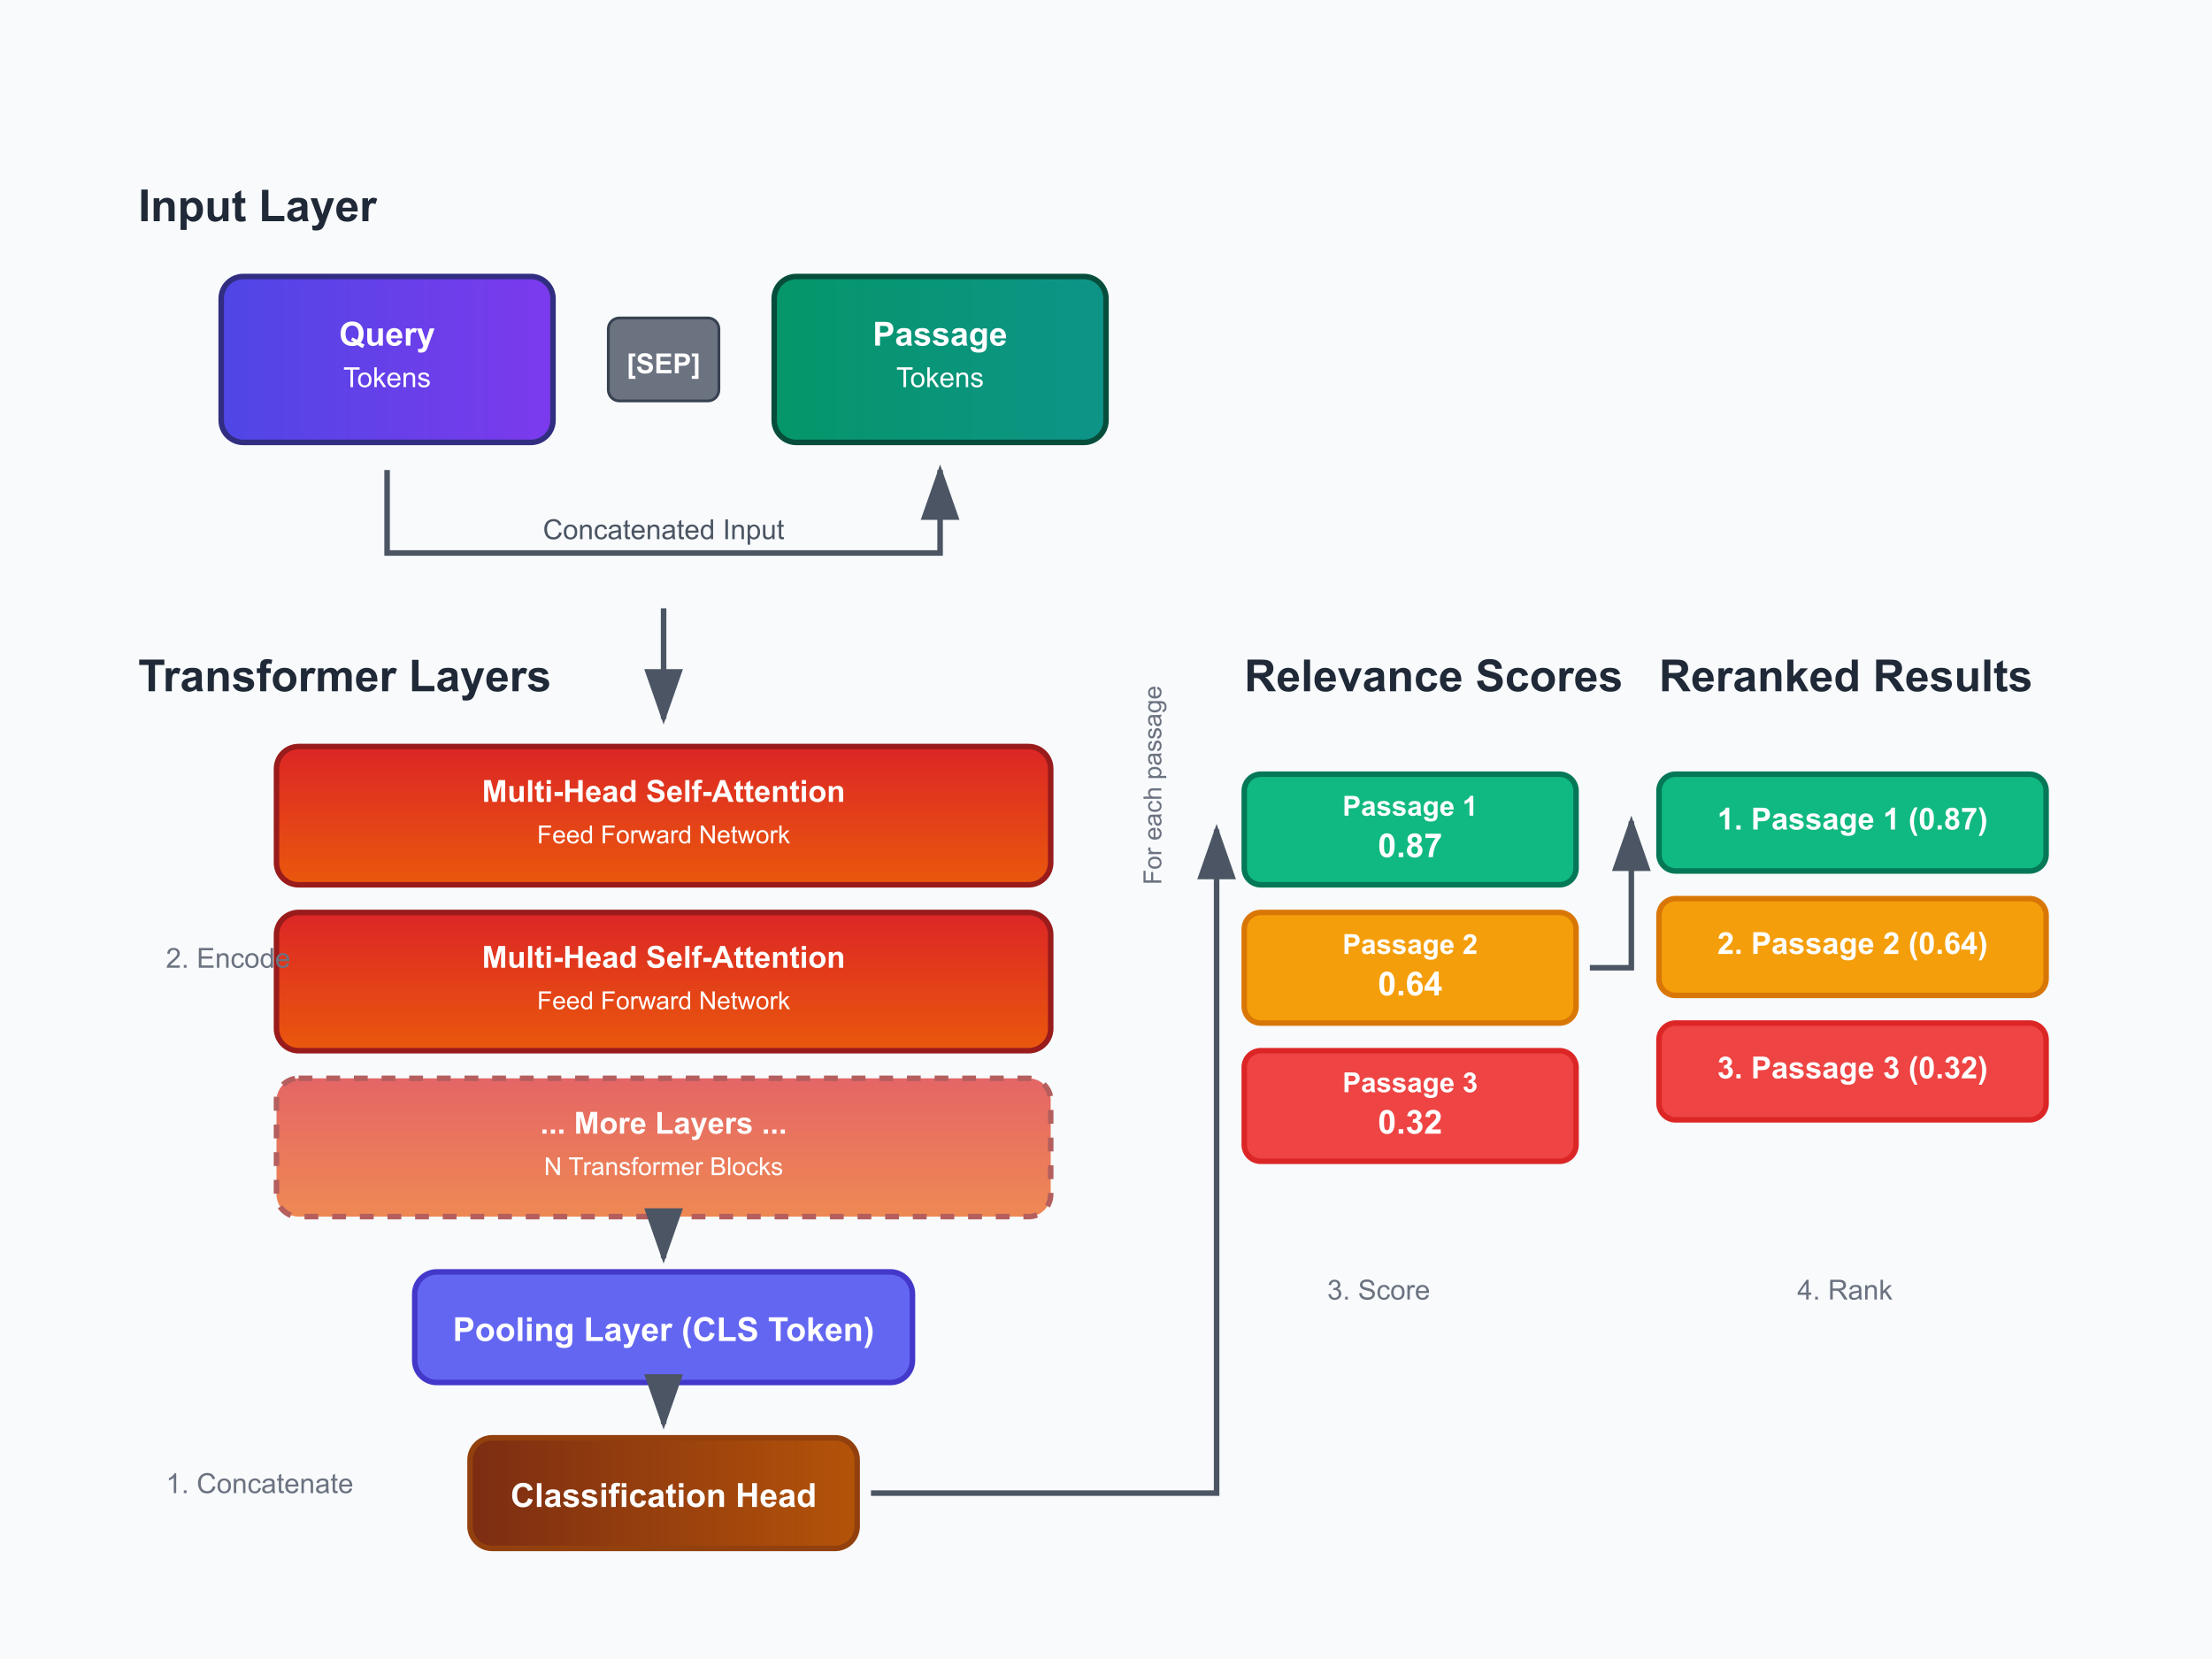
\includegraphics[width=\textwidth]{Figures/cross_encoder_diagram.png}
    \captionsetup{font=footnotesize, width=0.9\linewidth}
    \caption{Cross-Encoder Architecture for Passage Reranking. The model processes concatenated query-passage pairs through transformer layers, producing relevance scores for reranking candidate documents.}
    \label{fig:cross_encoder_architecture}
\end{figure}

The cross-encoder architecture follows a structured approach to relevance modeling:

\begin{enumerate}
    \item \textbf{Input Formatting}: Query and passage text are concatenated with special tokens: [CLS] query [SEP] passage [SEP]
    \item \textbf{Tokenization}: The input sequence is tokenized using subword tokenization (typically BERT-style WordPiece)
    \item \textbf{Transformer Encoding}: The concatenated sequence passes through multiple transformer layers with self-attention mechanisms
    \item \textbf{Relevance Prediction}: The [CLS] token representation is fed to a classification head producing a relevance score
    \item \textbf{Score Normalization}: Sigmoid activation ensures scores fall within [0,1] range for ranking
\end{enumerate}

\subsection{Model Architecture Specifications}

Three distinct transformer architectures were selected to represent different efficiency-effectiveness trade-offs:

\subsubsection{MiniLM-L12-H384-uncased}

MiniLM \cite{wang2020minilm} represents an efficient architecture designed through knowledge distillation:

\textbf{Architectural Parameters}:
\begin{itemize}
    \item Hidden dimensions: 384
    \item Number of layers: 12
    \item Attention heads: 12
    \item Maximum sequence length: 512 tokens
    \item Parameter count: ~33M parameters
    \item Vocabulary size: 30,522 tokens
\end{itemize}

\textbf{Design Philosophy}: MiniLM achieves efficiency through knowledge distillation from larger teacher models while maintaining competitive performance. The reduced hidden dimensions and moderate layer count make it suitable for resource-constrained scenarios while preserving essential language understanding capabilities.

\subsubsection{GTE-multilingual-base}

The General Text Embeddings (GTE) model \cite{li2023towards} extends capabilities to multilingual contexts with enhanced capacity:

\textbf{Architectural Parameters}:
\begin{itemize}
    \item Hidden dimensions: 768
    \item Number of layers: 12
    \item Attention heads: 12
    \item Maximum sequence length: 8192 tokens
    \item Parameter count: ~305M parameters
    \item Vocabulary size: 250,048 tokens
    \item Multilingual vocabulary support
\end{itemize}

\textbf{Design Philosophy}: GTE models are trained on diverse, multilingual corpora with multi-stage contrastive learning. The extended context length (8192 tokens) enables processing of longer documents, making it particularly suitable for comprehensive passage analysis and cross-lingual retrieval scenarios.

\subsubsection{ModernBERT-base}

ModernBERT \cite{modernbert} incorporates state-of-the-art architectural innovations for improved efficiency and effectiveness:

\textbf{Architectural Parameters}:
\begin{itemize}
    \item Hidden dimensions: 768
    \item Number of layers: 22
    \item Attention heads: 12
    \item Maximum sequence length: 8192 tokens
    \item Parameter count: ~149M parameters
    \item Vocabulary size: 50,368 tokens
    \item Advanced positional encoding and attention mechanisms
\end{itemize}

\textbf{Architectural Innovations}:
\begin{enumerate}
    \item \textbf{Rotary Position Embedding (RoPE)} \cite{su2023roformerenhancedtransformerrotary}: Enables effective handling of longer sequences through relative position encoding
    \item \textbf{Flash Attention} \cite{dao2022flashattentionfastmemoryefficientexact}: Improves memory efficiency and computational speed for attention operations
    \item \textbf{GeGLU Activation Functions} \cite{shazeer2020gluvariantsimprovetransformer}: Enhances model expressiveness while maintaining computational efficiency
\end{enumerate}

\textbf{Design Philosophy}: ModernBERT represents the current state-of-the-art in encoder-only transformers, combining architectural efficiency improvements with enhanced sequence processing capabilities. The deeper architecture (22 layers) with efficient attention mechanisms enables superior language understanding while maintaining practical computational requirements.

%----------------------------------------------------------------------------------------

\section{Optimizer Analysis and Implementation}

\subsection{AdamW Optimizer}

AdamW \cite{loshchilov2019decoupled} has established itself as the standard optimizer for transformer-based models through improved handling of weight decay regularization.

\subsubsection{Mathematical Formulation}

The AdamW update rule decouples weight decay from gradient-based updates:

\begin{align}
m_t &= \beta_1 m_{t-1} + (1 - \beta_1) g_t \\
v_t &= \beta_2 v_{t-1} + (1 - \beta_2) g_t^2 \\
\hat{m}_t &= \frac{m_t}{1 - \beta_1^t} \\
\hat{v}_t &= \frac{v_t}{1 - \beta_2^t} \\
\theta_t &= \theta_{t-1} - \eta \left( \frac{\hat{m}_t}{\sqrt{\hat{v}_t} + \epsilon} + \lambda \theta_{t-1} \right)
\end{align}

where:
\begin{itemize}
    \item $g_t$: gradient at time step $t$
    \item $m_t$: exponential moving average of gradients (momentum)
    \item $v_t$: exponential moving average of squared gradients
    \item $\eta$: learning rate
    \item $\lambda$: weight decay coefficient
    \item $\beta_1, \beta_2$: exponential decay rates for moment estimates
\end{itemize}

\subsubsection{Key Advantages}

\begin{enumerate}
    \item \textbf{Decoupled Weight Decay}: Separates regularization from adaptive learning rate scaling
    \item \textbf{Adaptive Learning Rates}: Per-parameter learning rate adaptation based on gradient history
    \item \textbf{Momentum Integration}: Incorporates momentum for improved convergence in consistent directions
    \item \textbf{Robustness}: Proven effectiveness across diverse transformer architectures and tasks
\end{enumerate}

\subsection{Lion Optimizer}

The Lion (Evolved Sign Momentum) optimizer \cite{chen2023symbolic} represents a novel approach discovered through symbolic mathematics and program search.

\subsubsection{Mathematical Formulation}

Lion utilizes a simplified update mechanism based on momentum and sign operations:

\begin{align}
c_t &= \beta_1 m_{t-1} + (1 - \beta_1) g_t \\
\theta_t &= \theta_{t-1} - \eta \left( \text{sign}(c_t) + \lambda \theta_{t-1} \right) \\
m_t &= \beta_2 m_{t-1} + (1 - \beta_2) g_t
\end{align}

where:
\begin{itemize}
    \item $c_t$: interpolated momentum for update direction
    \item $\text{sign}(\cdot)$: element-wise sign function
    \item Other parameters follow similar definitions as AdamW
\end{itemize}

\subsubsection{Key Innovations}

\begin{enumerate}
    \item \textbf{Sign-based Updates}: Uses only gradient direction, not magnitude, for parameter updates
    \item \textbf{Memory Efficiency}: Maintains only first-moment estimates, reducing memory requirements by ~50\%
    \item \textbf{Computational Simplicity}: Sign operation is computationally cheaper than square root calculations
    \item \textbf{Robust Performance}: Demonstrated effectiveness across computer vision and vision-language tasks
\end{enumerate}

\subsubsection{Theoretical Advantages}

The sign-based update mechanism provides several theoretical benefits:

\begin{itemize}
    \item \textbf{Noise Resistance}: Sign operation filters out gradient noise while preserving direction information
    \item \textbf{Scale Invariance}: Updates are independent of gradient magnitude, providing consistent step sizes
    \item \textbf{Convergence Properties}: Simplified dynamics may lead to more stable convergence in some scenarios
\end{itemize}

%----------------------------------------------------------------------------------------

\section{Training Framework and Implementation}

\subsection{Data Preprocessing and Input Formatting}

\subsubsection{Dataset Preparation}

The MS MARCO Passage Ranking dataset \cite{DBLP:journals/corr/NguyenRSGTMD16} serves as the primary training corpus:

\begin{itemize}
    \item \textbf{Training Queries}: 502,939 queries with relevance labels
    \item \textbf{Passage Collection}: 8.8M unique passages
    \item \textbf{Relevance Judgments}: Binary labels indicating passage relevance to queries
    \item \textbf{Data Source}: Real user queries from Bing search engine with human-annotated relevance
\end{itemize}

\subsubsection{Input Processing Pipeline}

\textbf{Text Preprocessing}:
\begin{enumerate}
    \item Unicode normalization and cleaning
    \item Whitespace normalization
    \item Special character handling for robustness
\end{enumerate}

\textbf{Sequence Construction}:
\begin{enumerate}
    \item Query-passage concatenation: [CLS] query [SEP] passage [SEP]
    \item Tokenization using model-specific tokenizers
    \item Sequence length truncation based on model capacity
    \item Attention mask creation for proper sequence processing
\end{enumerate}

\textbf{Batch Construction}:
\begin{enumerate}
    \item Dynamic padding to maximum sequence length in batch
    \item Label tensor creation for binary classification
    \item Efficient DataLoader implementation with multi-processing
\end{enumerate}

\subsection{Training Configuration}

\subsubsection{Hyperparameter Settings}

\textbf{Model-Specific Configurations}:

\begin{table}[h!]
\centering
\begin{tabular}{|l|c|c|c|}
\hline
\textbf{Parameter} & \textbf{MiniLM} & \textbf{GTE} & \textbf{ModernBERT} \\
\hline
Learning Rate & 2e-5 & 2e-5 & 2e-6 \\
\hline
Max Sequence Length & 512 & 8192 & 8192 \\
\hline
Batch Size & 16 & 16 & 16 \\
\hline
Weight Decay & 0.01 & 0.01 & 0.01 \\
\hline
Warmup Steps & 1000 & 1000 & 1000 \\
\hline
LR Scheduler & None & None & Cosine Annealing \\
\hline
Training Epochs & 3 & 3 & 3 \\
\hline
\end{tabular}
\caption{Model-specific training configurations for optimal performance}
\label{tab:training_config}
\end{table}

\textbf{Optimizer-Specific Parameters}:

\begin{table}[h!]
\centering
\begin{tabular}{|l|c|c|}
\hline
\textbf{Parameter} & \textbf{AdamW} & \textbf{Lion} \\
\hline
$\beta_1$ & 0.9 & 0.9 \\
\hline
$\beta_2$ & 0.999 & 0.99 \\
\hline
$\epsilon$ & 1e-8 & - \\
\hline
Gradient Clipping & 1.0 & 1.0 \\
\hline
\end{tabular}
\caption{Optimizer-specific parameter configurations}
\label{tab:optimizer_config}
\end{table}

\subsubsection{Training Objectives}

\textbf{Loss Function}: Binary Cross-Entropy Loss for relevance prediction:

\begin{equation}
\mathcal{L}_{BCE} = -\frac{1}{N} \sum_{i=1}^{N} [y_i \log(\hat{y}_i) + (1-y_i) \log(1-\hat{y}_i)]
\end{equation}

where $y_i$ represents the true relevance label and $\hat{y}_i$ is the predicted relevance score.

\textbf{Regularization Strategies}:
\begin{itemize}
    \item Weight decay regularization (L2 penalty)
    \item Gradient clipping for training stability
    \item Early stopping based on validation performance
\end{itemize}

\subsection{Infrastructure and Implementation}

\subsubsection{Computational Resources}

\textbf{Hardware Platform}: Modal cloud computing platform \cite{modal_labs}
\begin{itemize}
    \item GPU: NVIDIA A100-80GB
    \item Memory: High-bandwidth memory for large model training
    \item Storage: Fast SSD storage for efficient data loading
    \item Network: High-speed interconnects for distributed training
\end{itemize}

\textbf{Software Stack}:
\begin{itemize}
    \item Framework: PyTorch \cite{paszke2019pytorchimperativestylehighperformance}
    \item Model Library: Sentence Transformers \cite{reimers2019sentence}
    \item Evaluation Tools: TREC Eval \cite{trec_eval_github}, Pyserini \cite{lin2021pyserini}
    \item Experiment Tracking: Weights \& Biases \cite{wandb2020}
\end{itemize}

\subsubsection{Training Pipeline}

\textbf{Model Initialization}:
\begin{enumerate}
    \item Load pre-trained transformer weights
    \item Initialize classification head for relevance prediction
    \item Set up optimizer with appropriate hyperparameters
    \item Configure learning rate scheduler if applicable
\end{enumerate}

\textbf{Training Loop}:
\begin{enumerate}
    \item Forward pass through cross-encoder model
    \item Compute binary cross-entropy loss
    \item Backward propagation with gradient computation
    \item Optimizer step with gradient clipping
    \item Learning rate scheduling update
    \item Validation evaluation at specified intervals
\end{enumerate}

\textbf{Model Checkpointing}:
\begin{itemize}
    \item Save model state at each epoch
    \item Track best model based on validation metrics
    \item Enable training resumption from checkpoints
    \item Model versioning for reproducibility
\end{itemize}

This comprehensive training framework ensures consistent and reproducible comparison between Lion and AdamW optimizers across different model architectures while maintaining state-of-the-art training practices for cross-encoder models in information retrieval.


\section{Implementation Considerations}

\subsection{Computational Resources}
The experimental setup requires significant computational resources due to the intensive nature of cross-encoder training. Modal cloud platform provides the necessary GPU resources with NVIDIA A100 instances, ensuring consistent hardware configuration across all experiments.

Resource allocation considerations include:
\begin{itemize}
    \item GPU memory requirements varying by model size (8GB for MiniLM, 16GB for GTE, 24GB for ModernBERT)
    \item Batch size optimization based on available memory
    \item Distributed training capabilities for larger models
    \item Checkpoint storage and management
\end{itemize}

\subsection{Reproducibility Framework}
Ensuring reproducible results across different runs and environments requires careful attention to:

\textbf{Random Seed Management}:
\begin{itemize}
    \item Fixed seeds for PyTorch, NumPy, and Python random modules
    \item Deterministic CUDA operations where possible
    \item Consistent data shuffling across experiments
\end{itemize}

\textbf{Environment Specification}:
\begin{itemize}
    \item Docker containerization for consistent software environments
    \item Dependency version pinning in requirements files
    \item Hardware specification documentation
    \item Environment variable standardization
\end{itemize}

\subsection{Evaluation Pipeline}
The evaluation pipeline ensures consistent and fair comparison between optimizers:

\textbf{Model Loading and Inference}:
\begin{itemize}
    \item Standardized model loading procedures
    \item Consistent tokenization and preprocessing
    \item Batch size optimization for inference efficiency
    \item GPU memory management during evaluation
\end{itemize}

\textbf{Metric Computation}:
\begin{itemize}
    \item Implementation of standard IR metrics (nDCG, MAP, MRR)
    \item Statistical significance testing procedures
    \item Result aggregation and reporting mechanisms
    \item Cross-validation protocols for robust evaluation
\end{itemize}

\section{Chapter Summary}

This chapter presented a comprehensive methodology for comparing Lion and AdamW optimizers in cross-encoder architectures for information retrieval. The systematic approach encompasses model architecture specifications, optimizer implementations, training frameworks, and evaluation protocols.

Key methodological contributions include:

\begin{itemize}
    \item \textbf{Systematic Architecture Comparison}: Detailed specifications for MiniLM, GTE, and ModernBERT cross-encoder implementations, enabling fair comparison across different model scales and designs.
    
    \item \textbf{Rigorous Optimizer Implementation}: Mathematical formulations and computational implementations of both Lion and AdamW optimizers, ensuring consistent comparison conditions.
    
    \item \textbf{Standardized Training Protocol}: Comprehensive training framework with hyperparameter optimization, regularization strategies, and monitoring systems for reproducible results.
    
    \item \textbf{Robust Evaluation Framework}: Multi-dataset evaluation protocol using TREC 2019 and MS MARCO benchmarks with statistical significance testing.
\end{itemize}

The methodology establishes a foundation for systematic optimizer comparison in neural information retrieval, providing insights into the relationship between optimization algorithms and model architectures. The next chapter presents the comprehensive experimental results obtained through this methodological framework.
 


\chapter{Results and Performance Analysis}
\label{Chapter5}

This chapter presents a comprehensive analysis of our experimental results comparing the Lion and AdamW optimizers for cross-encoder reranking models. We evaluate three distinct transformer architectures (MiniLM, GTE, and ModernBERT) across multiple metrics and examine their training dynamics through detailed visualizations.

\section{Experimental Results}

\subsection{Main Performance Metrics}

Table~\ref{tab:main_results} presents the comprehensive evaluation results for all model configurations on both the TREC 2019 Deep Learning Track and MS MARCO development set. The results are tracked across three training epochs for each model-optimizer combination.

\begin{table*}[htbp]
\centering
\caption{Evaluation Results on TREC-DL 2019 and MS-MARCO Dev Passage Ranking}
\label{tab:main_results}
\resizebox{\textwidth}{!}{%
\begin{tabular}{l l c c c c c c c}
\toprule
\textbf{Base Model} & \textbf{Optimizer} & \textbf{Epoch} & \textbf{NDCG@10} & \textbf{MAP} & \textbf{MRR@10} & \textbf{Recall@10} & \textbf{R-Prec} & \textbf{P@10} \\
\midrule
\multirow{3}{*}{MiniLM-L12-H384} & \multirow{3}{*}{AdamW}
    & 1 & 0.7008 & 0.4814 & 0.5828 & 0.1712 & 0.4899 & 0.8047 \\
    & & 2 & 0.7094 & 0.4891 & 0.5818 & 0.1715 & 0.5017 & 0.8093 \\
    & & 3 & 0.7127 & 0.4908 & 0.5826 & 0.1706 & 0.4962 & 0.8023 \\
\midrule
\multirow{3}{*}{MiniLM-L12-H384} & \multirow{3}{*}{Lion}
    & 1 & 0.7031 & 0.4858 & 0.5890 & 0.1698 & 0.4904 & 0.8070 \\
    & & 2 & 0.6916 & 0.4755 & 0.5942 & 0.1724 & 0.5041 & 0.8116 \\
    & & 3 & 0.6808 & 0.4706 & \cellcolor{yellow!50}\textbf{0.5988} & 0.1701 & 0.4923 & 0.8023 \\
\midrule
\multirow{3}{*}{GTE-multilingual-base} & \multirow{3}{*}{AdamW}
    & 1 & 0.7224 & 0.5005 & 0.5940 & 0.1733 & 0.4957 & 0.8140 \\
    & & 2 & 0.7203 & 0.4999 & 0.5942 & \cellcolor{yellow!50}\textbf{0.1733} & 0.5067 & 0.8163 \\
    & & 3 & 0.6902 & 0.4899 & 0.5972 & 0.1730 & 0.5069 & 0.8140 \\
\midrule
\multirow{3}{*}{GTE-multilingual-base} & \multirow{3}{*}{Lion}
    & 1 & 0.6785 & 0.4754 & 0.5854 & 0.1684 & 0.4849 & 0.7953 \\
    & & 2 & 0.6909 & 0.4921 & 0.5957 & 0.1721 & 0.5053 & 0.8140 \\
    & & 3 & 0.6904 & 0.4912 & 0.5931 & 0.1719 & 0.5041 & 0.8093 \\
\midrule
\multirow{3}{*}{Modern-BERT-base} & \multirow{3}{*}{AdamW}
    & 1 & 0.7105 & 0.5066 & 0.5865 & 0.1678 & 0.5161 & 0.8163 \\
    & & 2 & 0.6839 & 0.4893 & 0.5885 & 0.1634 & 0.4946 & 0.7814 \\
    & & 3 & 0.6959 & 0.4971 & 0.5916 & 0.1623 & 0.5116 & 0.7860 \\ % Corrected P@10 based on context
\midrule
\multirow{3}{*}{Modern-BERT-base} & \multirow{3}{*}{Lion}
    & 1 & 0.7142 & \cellcolor{yellow!50}\textbf{0.5121} & 0.5834 & 0.1689 & 0.5148 & 0.8163 \\
    & & 2 & \cellcolor{yellow!50}\textbf{0.7225} & 0.5115 & 0.5907 & 0.1732 & \cellcolor{yellow!50}\textbf{0.5183} & 0.8209 \\
    & & 3 & 0.7051 & 0.5020 & \cellcolor{yellow!50}\textbf{0.5988}* & 0.1722 & 0.5102 & \cellcolor{yellow!50}\textbf{0.8256} \\
\bottomrule
\end{tabular}%
}
\vspace{1em}\\
\footnotesize{* MRR@10 is calculated on the MS MARCO v1.1 passage dataset development split. All other metrics are calculated on TREC DL 2019. Best result for each metric highlighted. (*Note: MiniLM+Lion also achieved 0.5988 MRR@10 at epoch 3, see Appendix~\ref{AppendixA} for complete metrics).}
\end{table*}

\subsection{Training Dynamics Analysis}

To better understand the behavior of each optimizer-model combination, we analyze their training dynamics through various metrics. The following figures present comparative visualizations of training trajectories.

\subsubsection{ModernBERT Training Dynamics}

\begin{figure}[H]
    \centering
    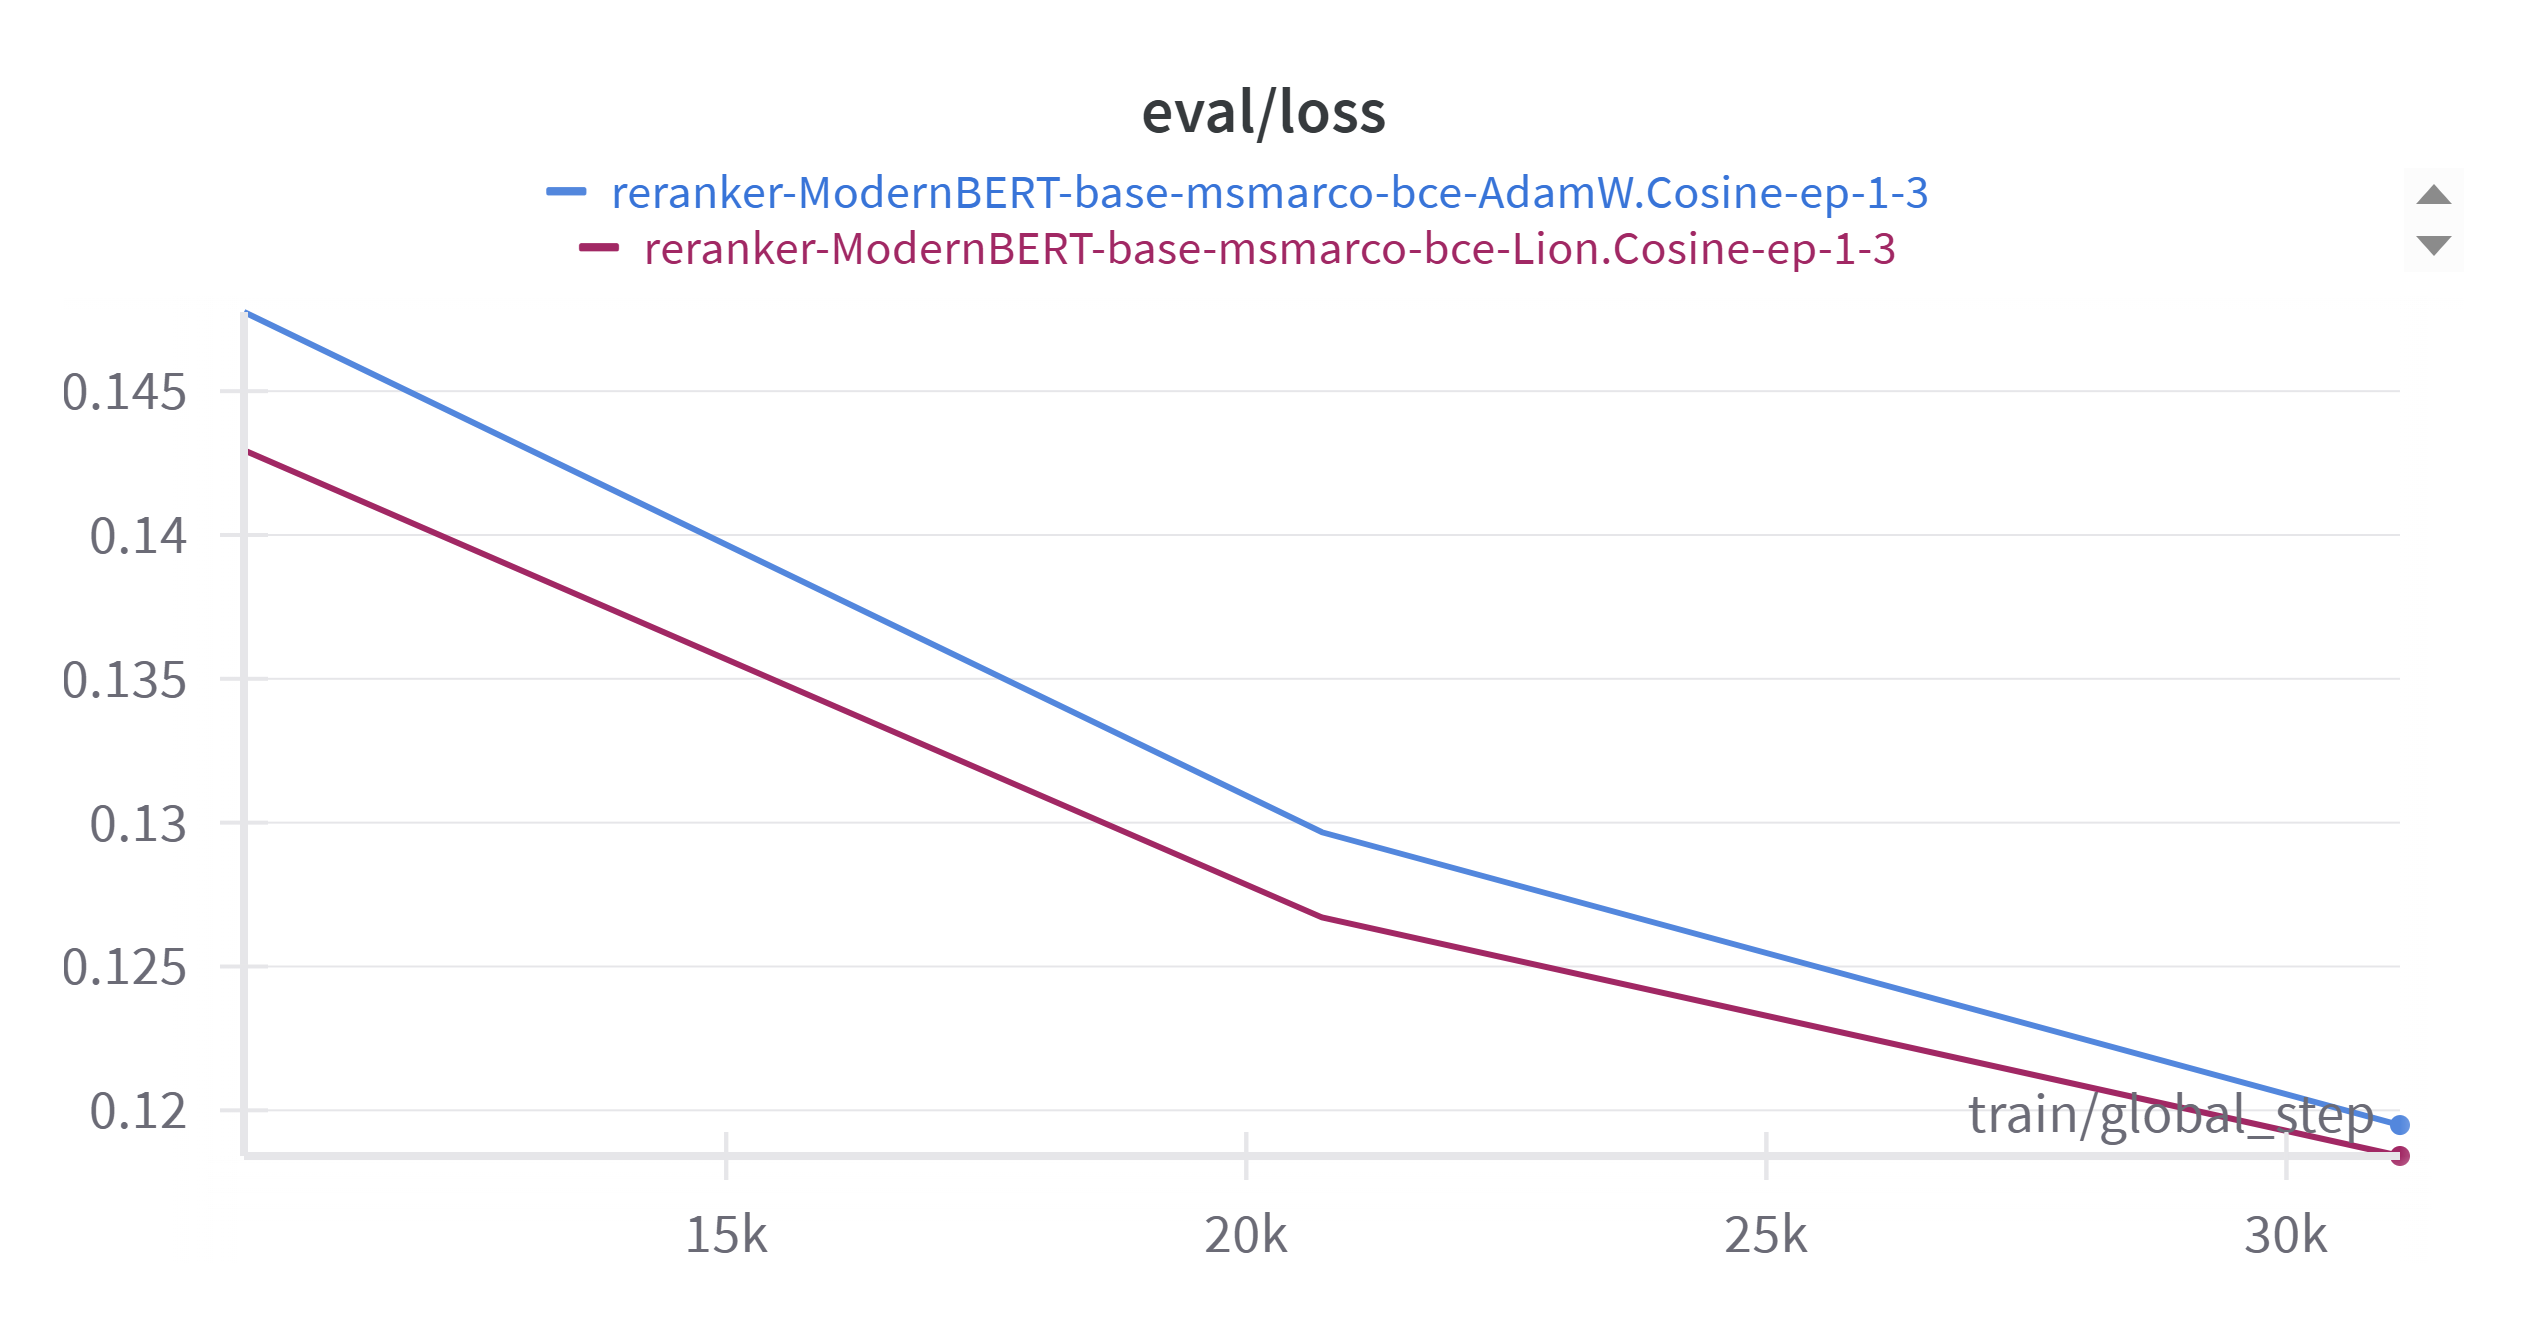
\includegraphics[width=0.8\textwidth]{Figures/modernBERT-Lion-AdamW-eval_loss.png}
    \caption{ModernBERT: Evaluation Loss Comparison between Lion and AdamW}
    \label{fig:modernbert_eval_loss}
\end{figure}

\begin{figure}[H]
    \centering
    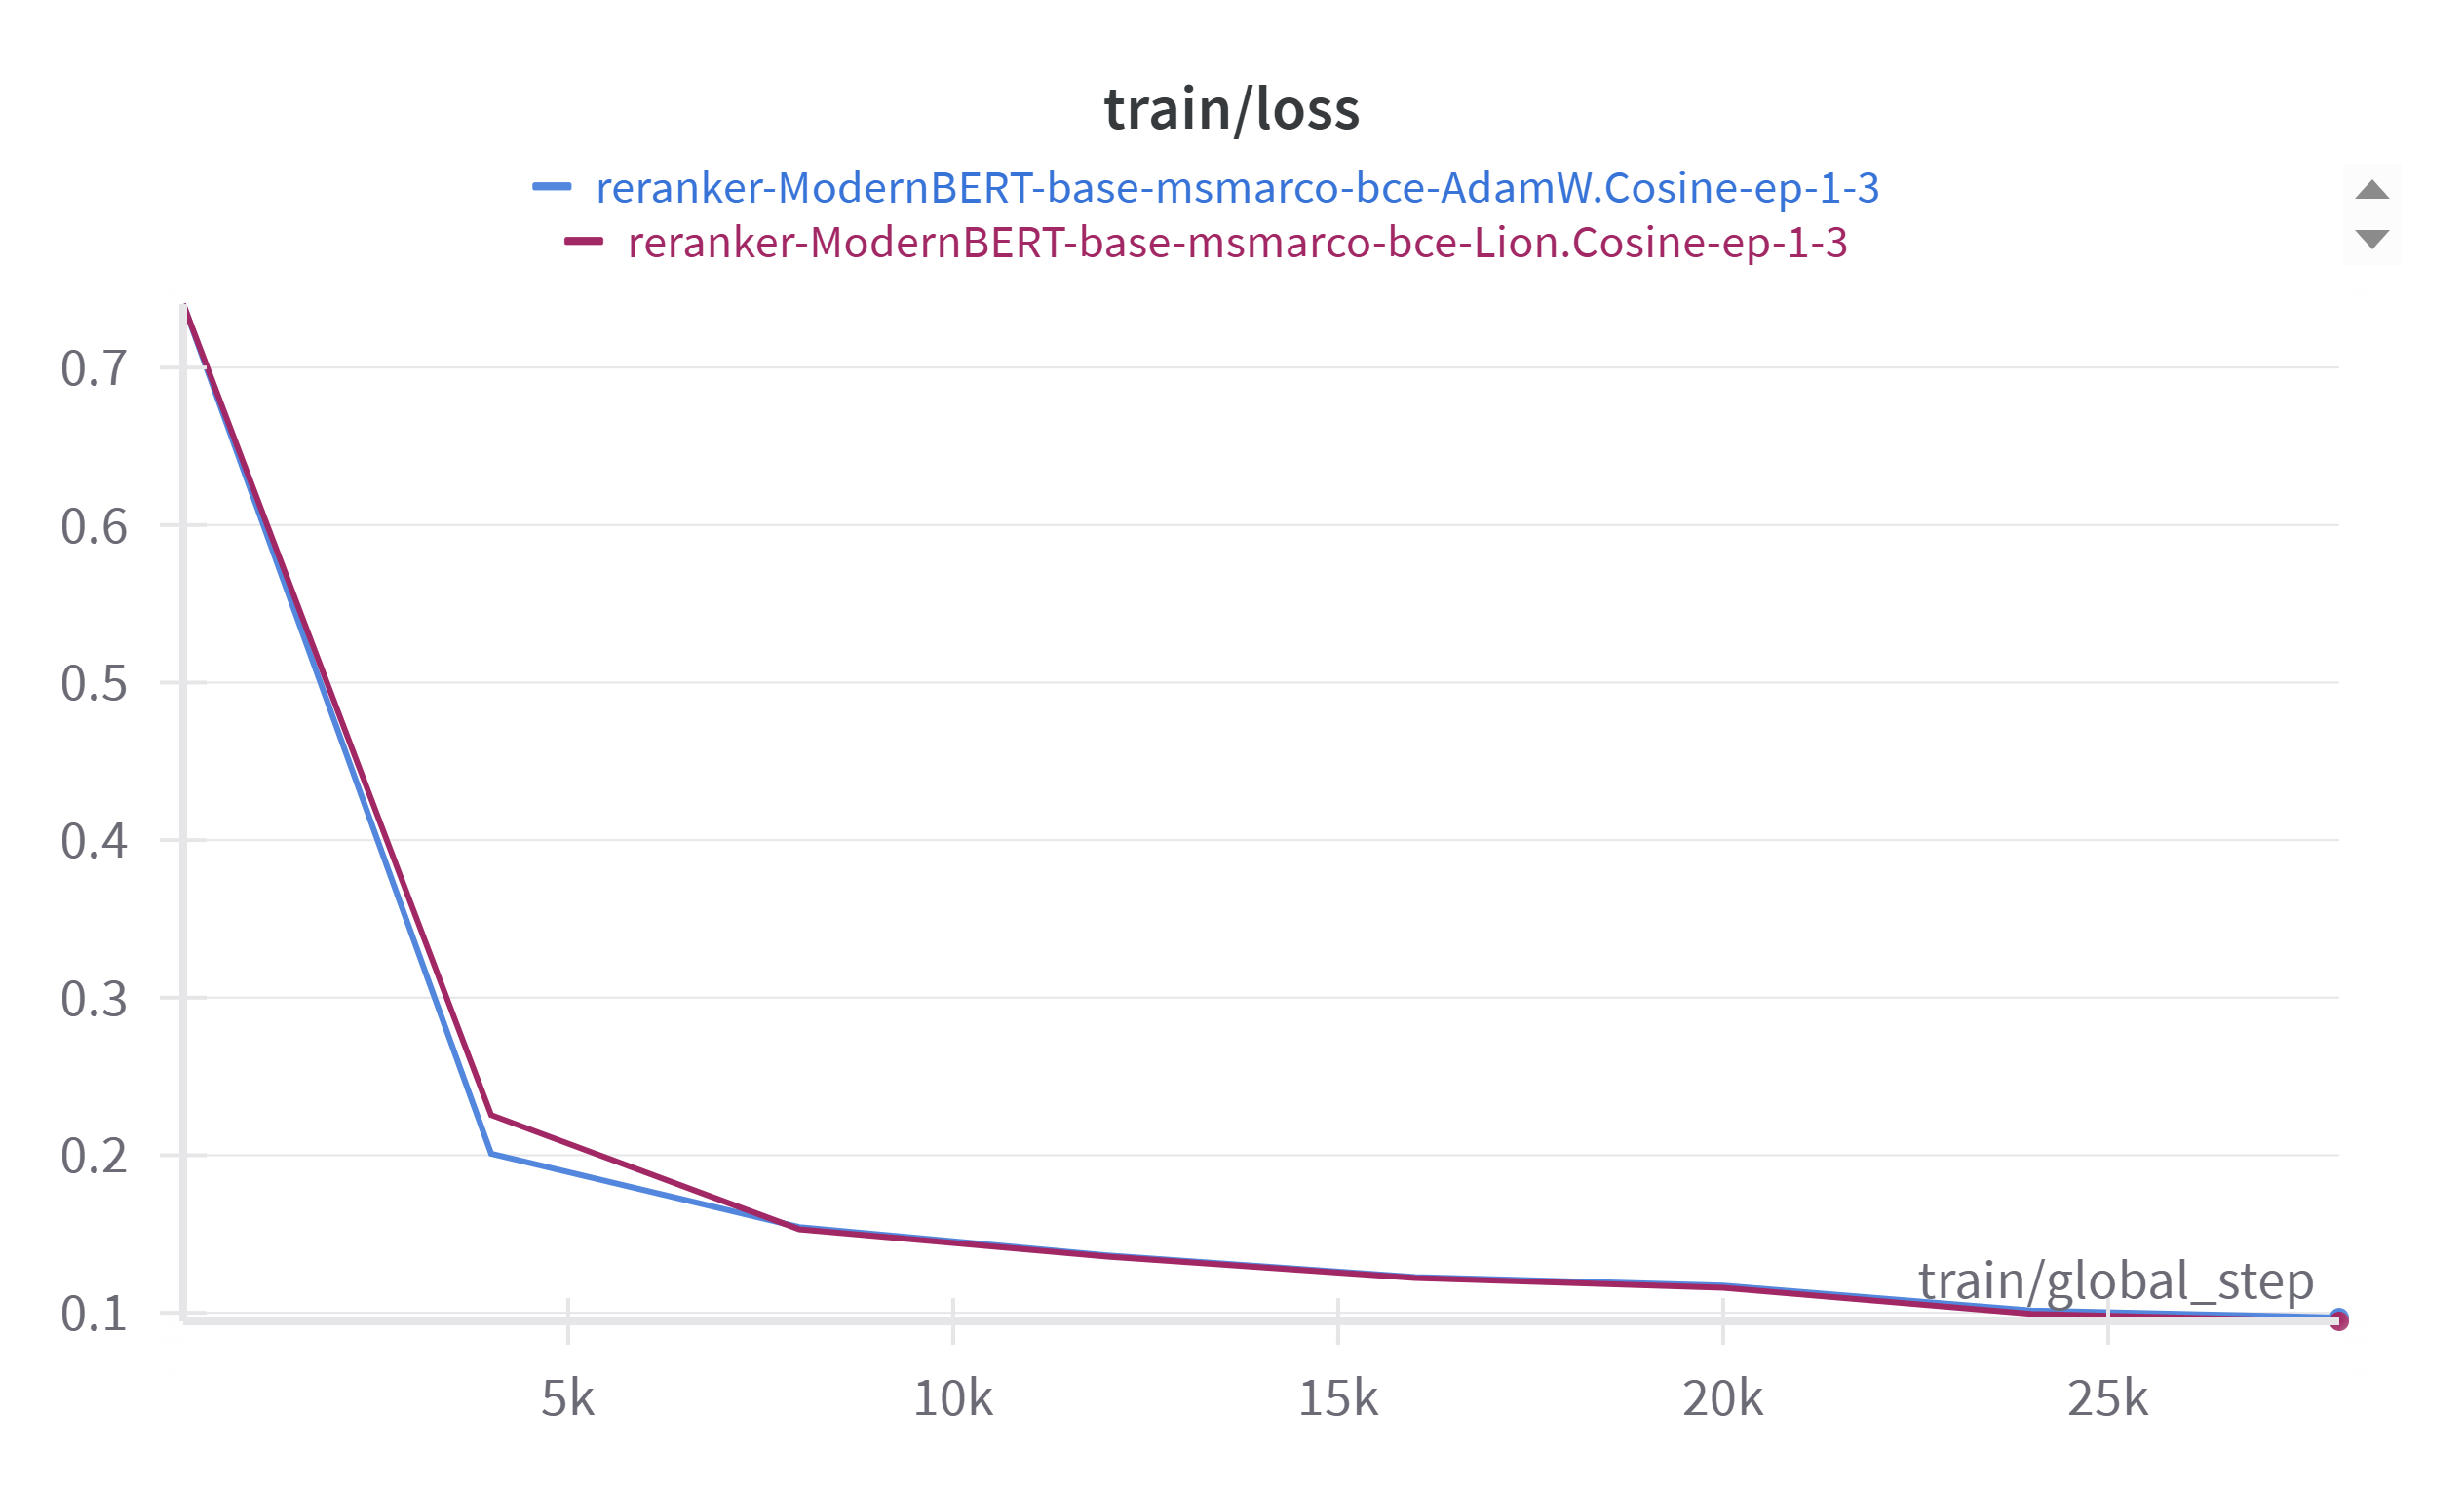
\includegraphics[width=0.8\textwidth]{Figures/modernBERT-Lion-adamW-train_loss.png}
    \caption{ModernBERT: Training Loss Progression}
    \label{fig:modernbert_train_loss}
\end{figure}

\begin{figure}[H]
    \centering
    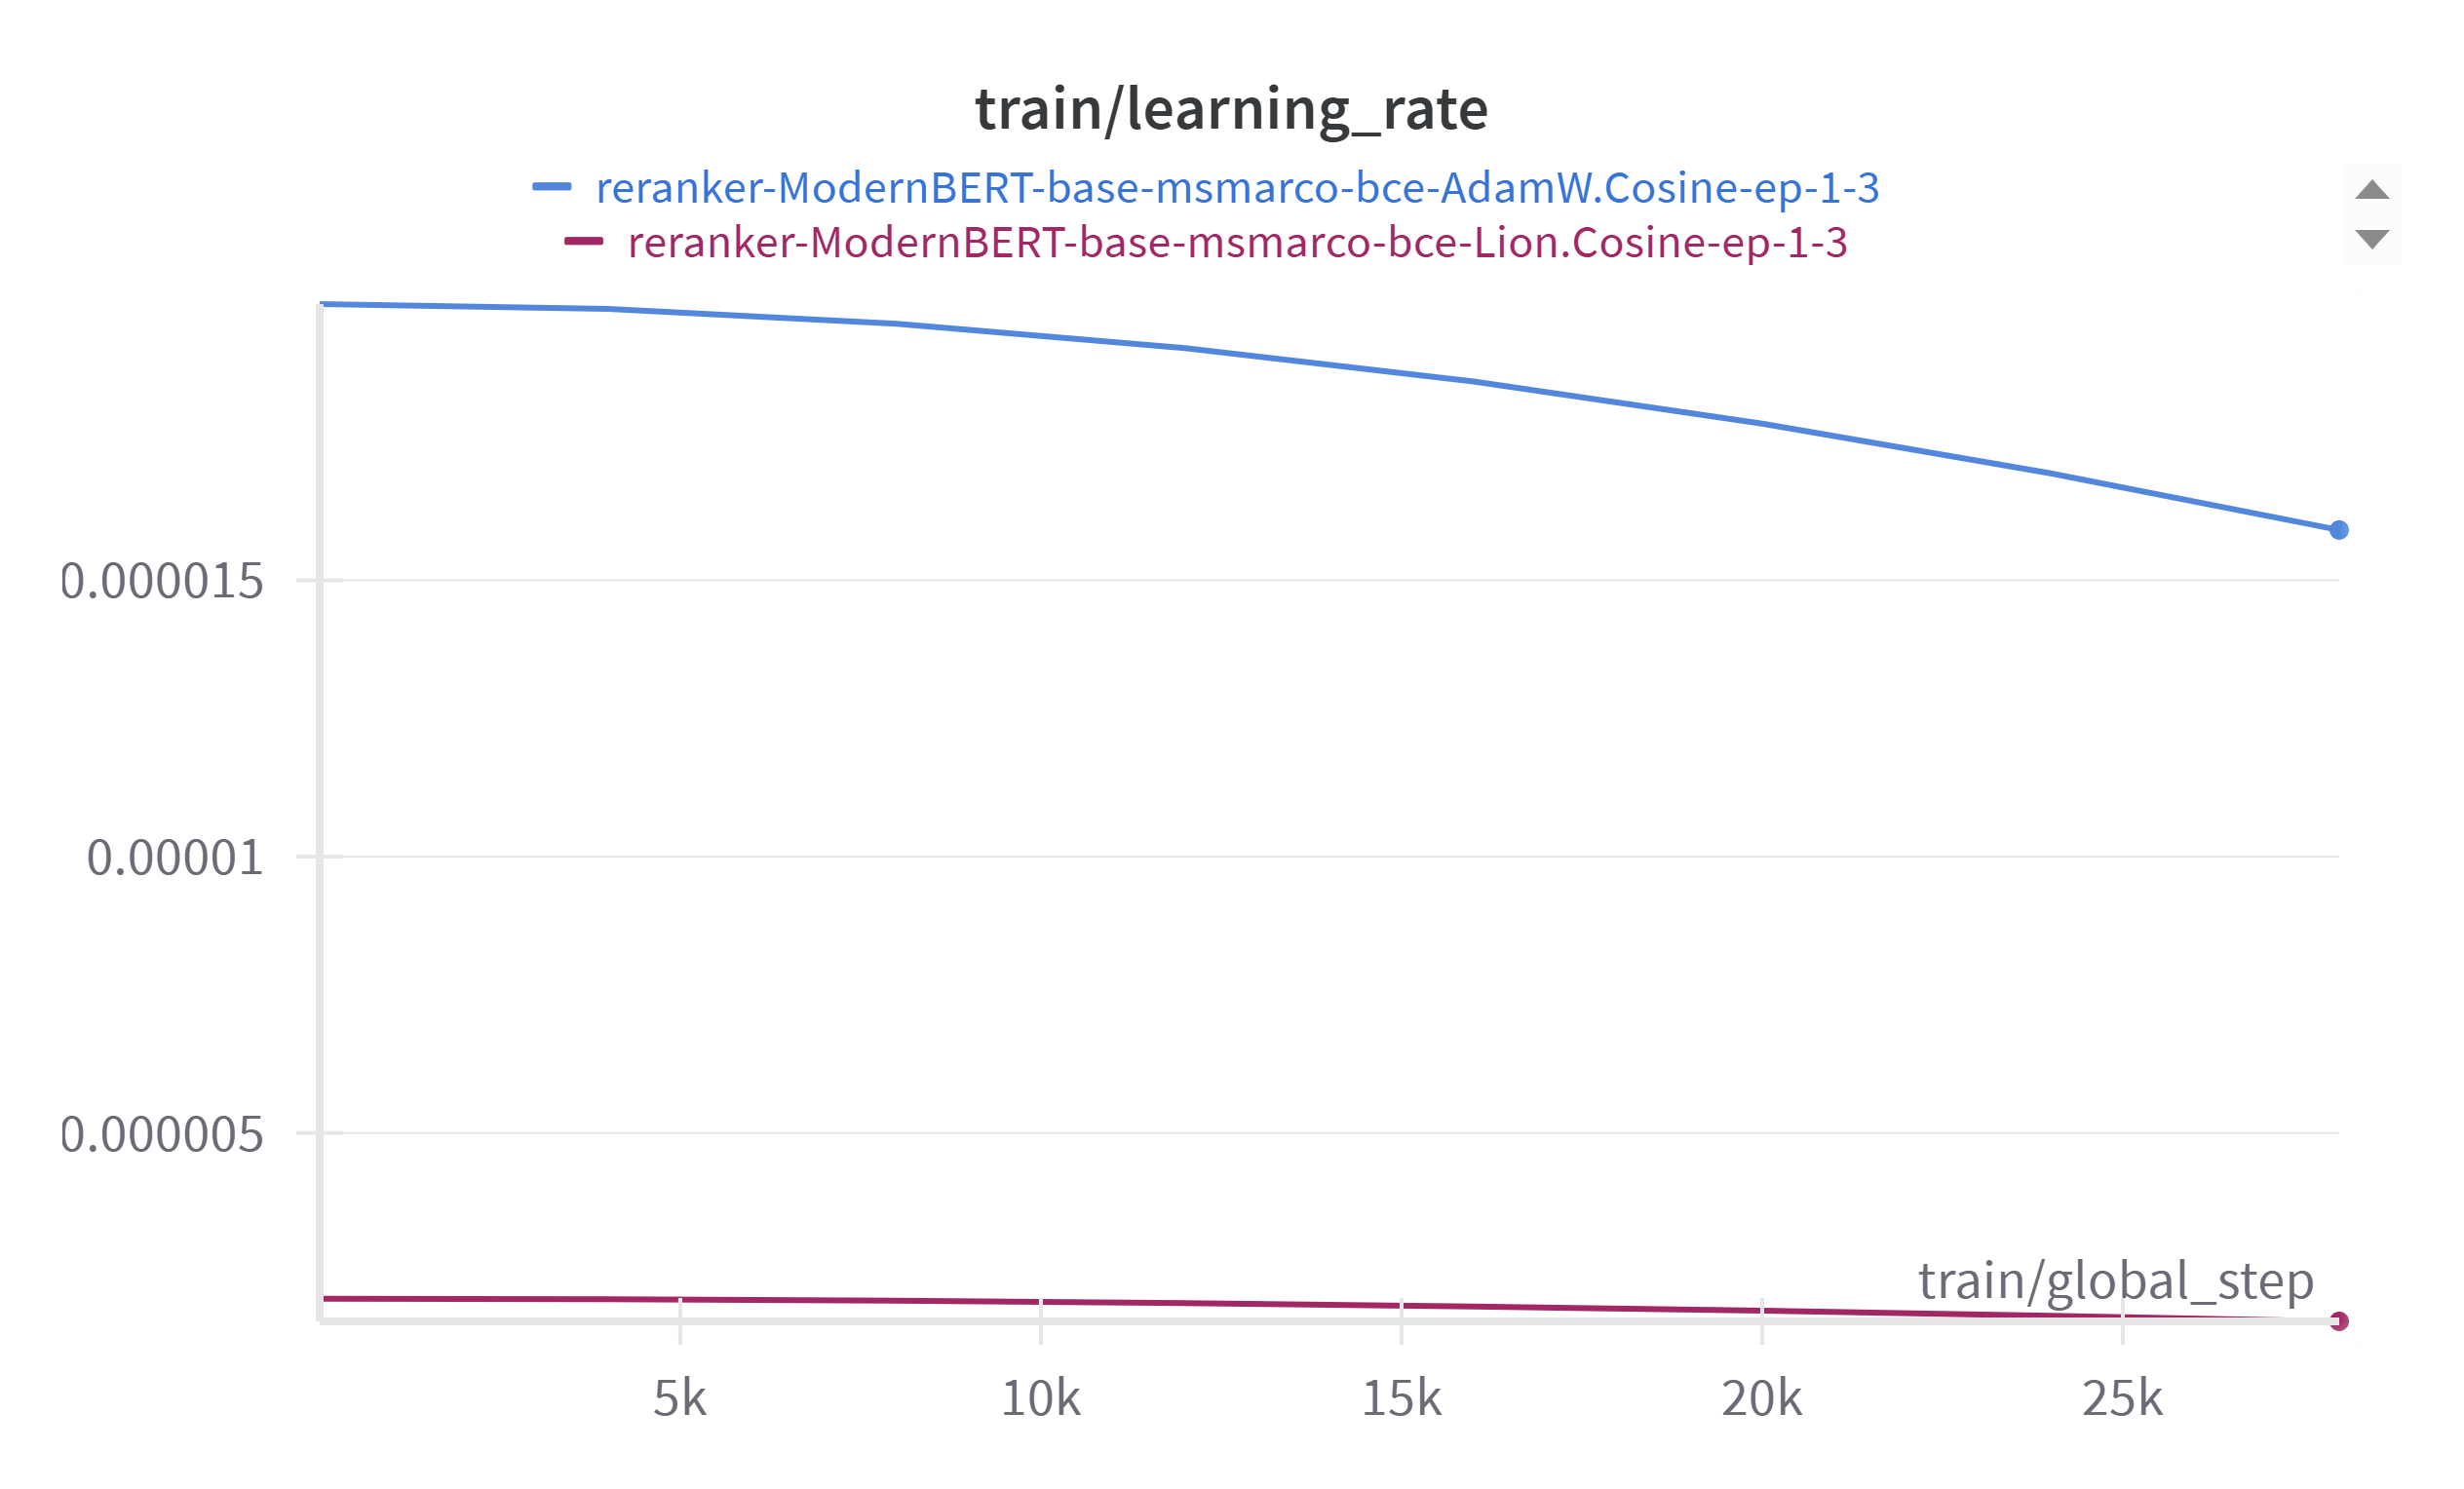
\includegraphics[width=0.8\textwidth]{Figures/modernBERT-Lion-adamW-lrate.png}
    \caption{ModernBERT: Learning Rate Schedule}
    \label{fig:modernbert_lr}
\end{figure}

\begin{figure}[H]
    \centering
    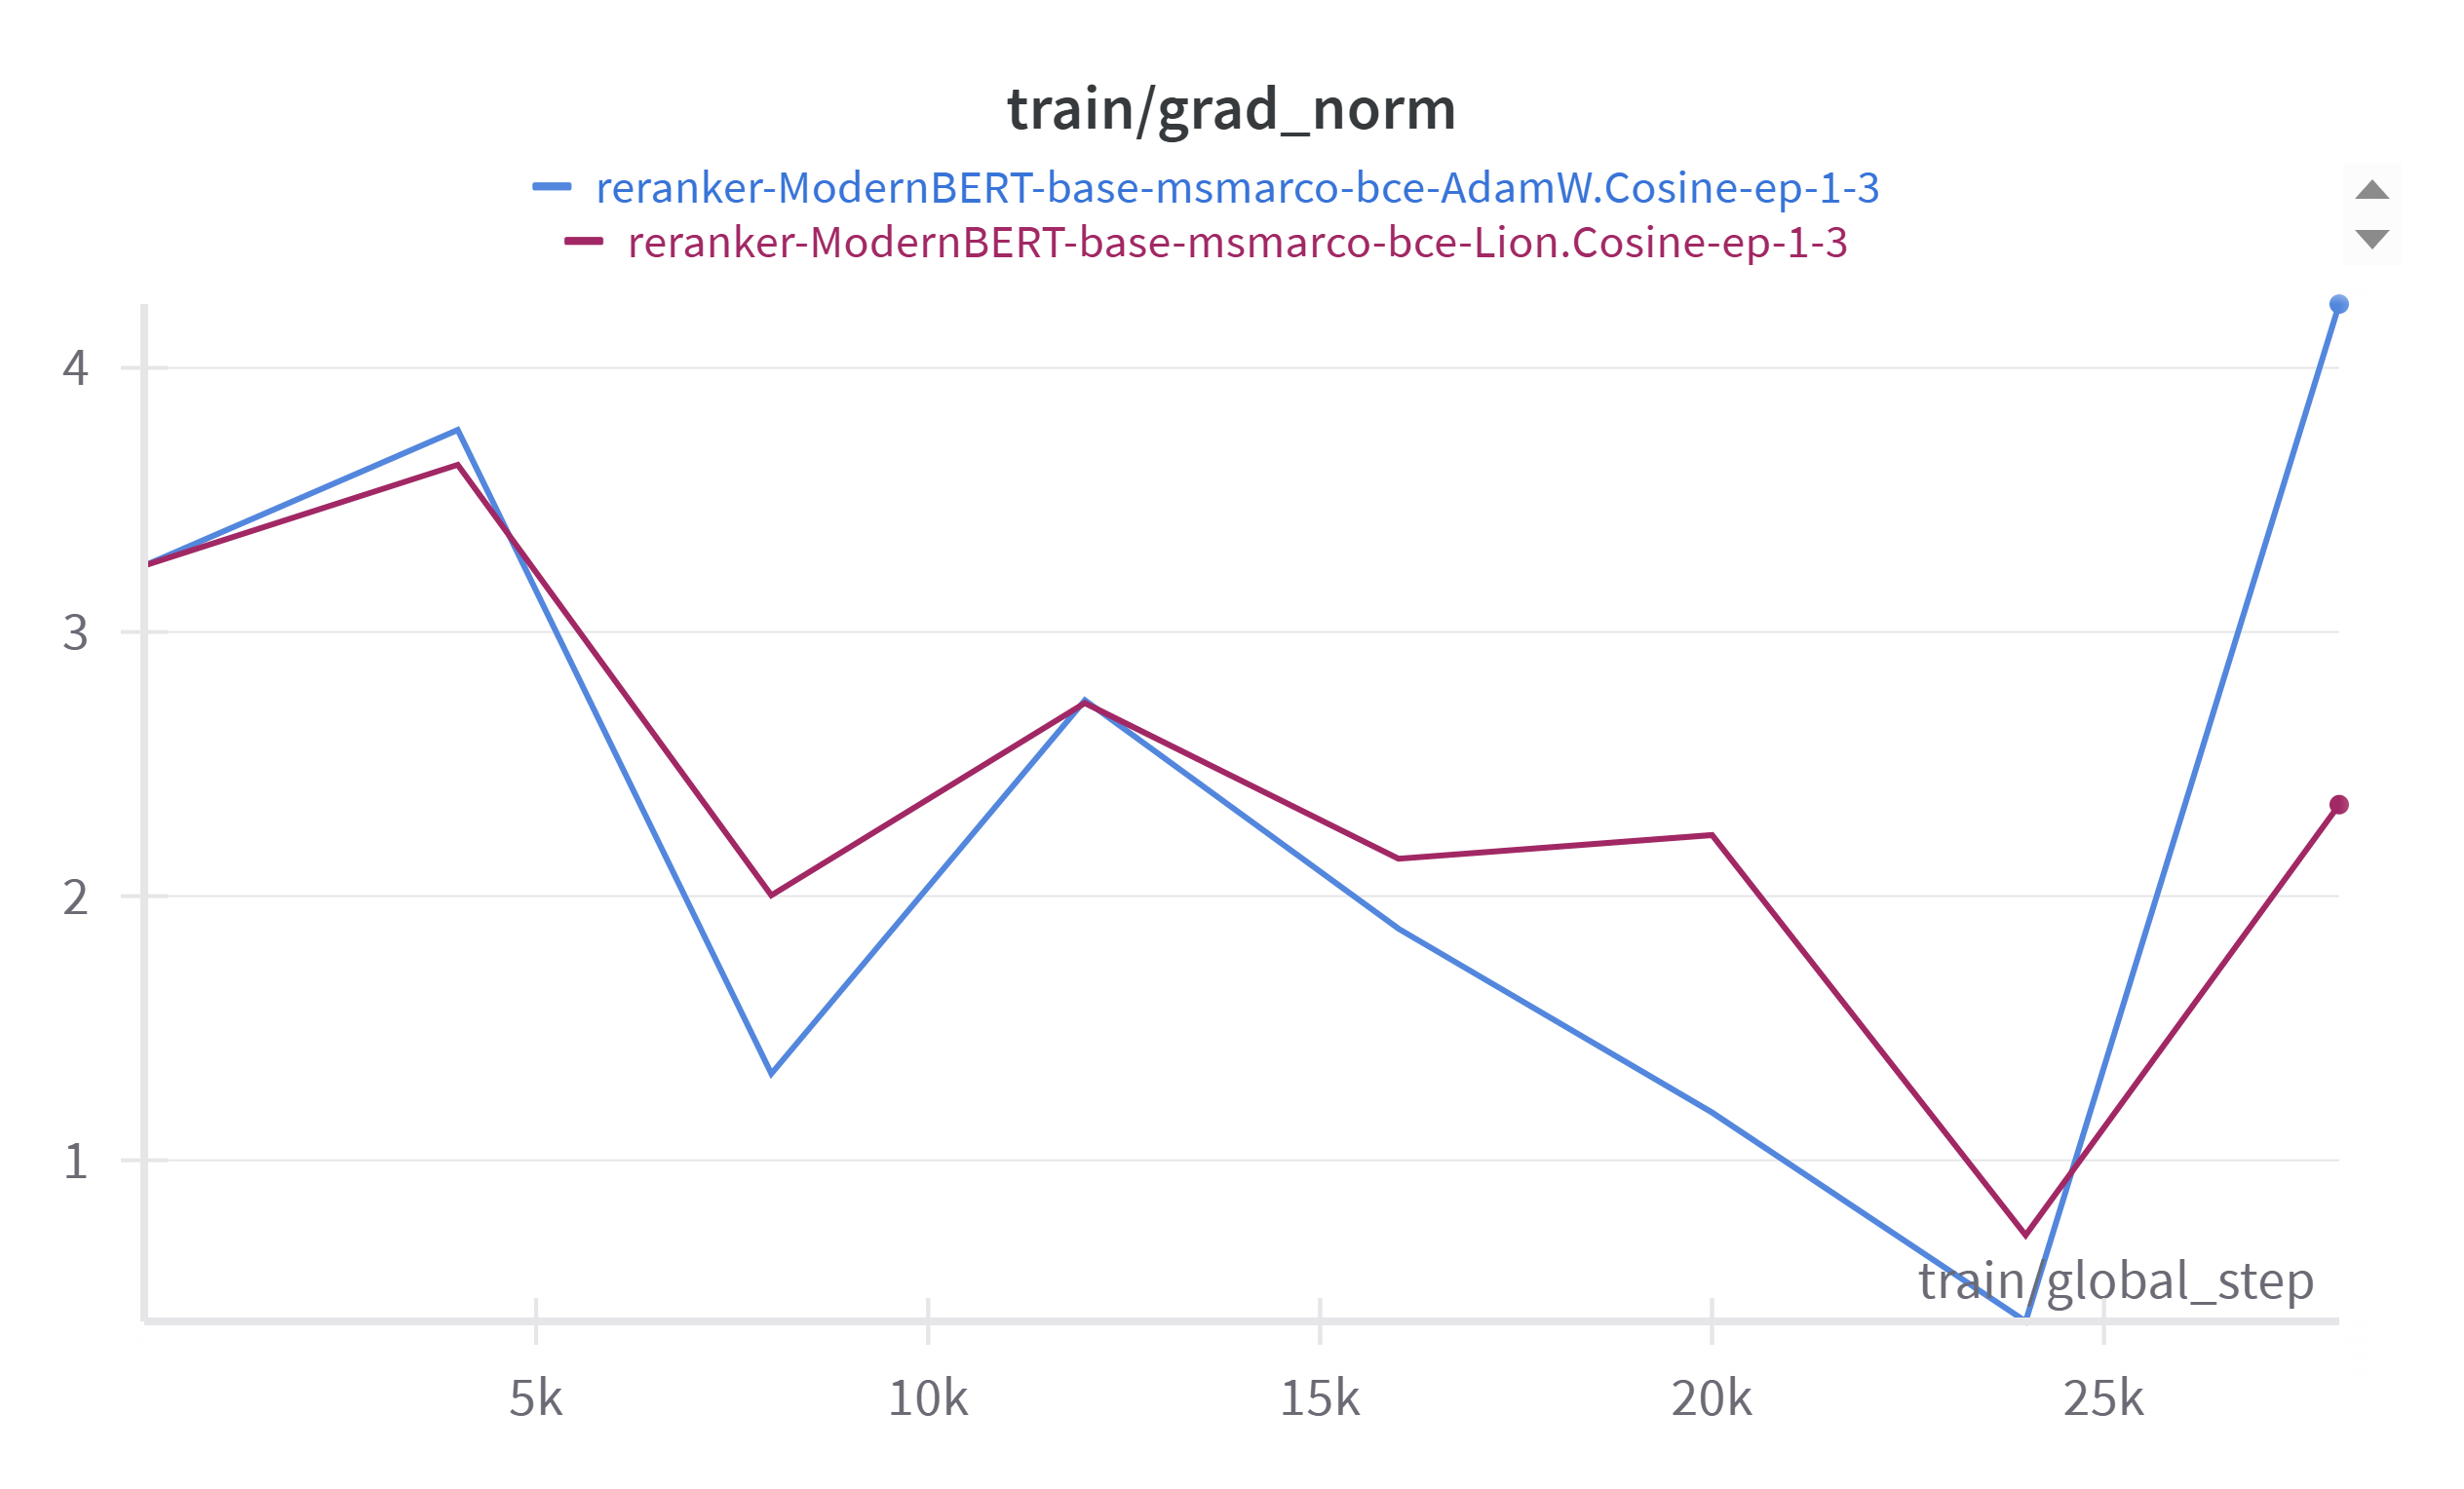
\includegraphics[width=0.8\textwidth]{Figures/modernBERT-Lion-adamW_grad_norm.png}
    \caption{ModernBERT: Gradient Norm Evolution}
    \label{fig:modernbert_grad_norm}
\end{figure}

\subsubsection{GTE Training Dynamics}

\begin{figure}[H]
    \centering
    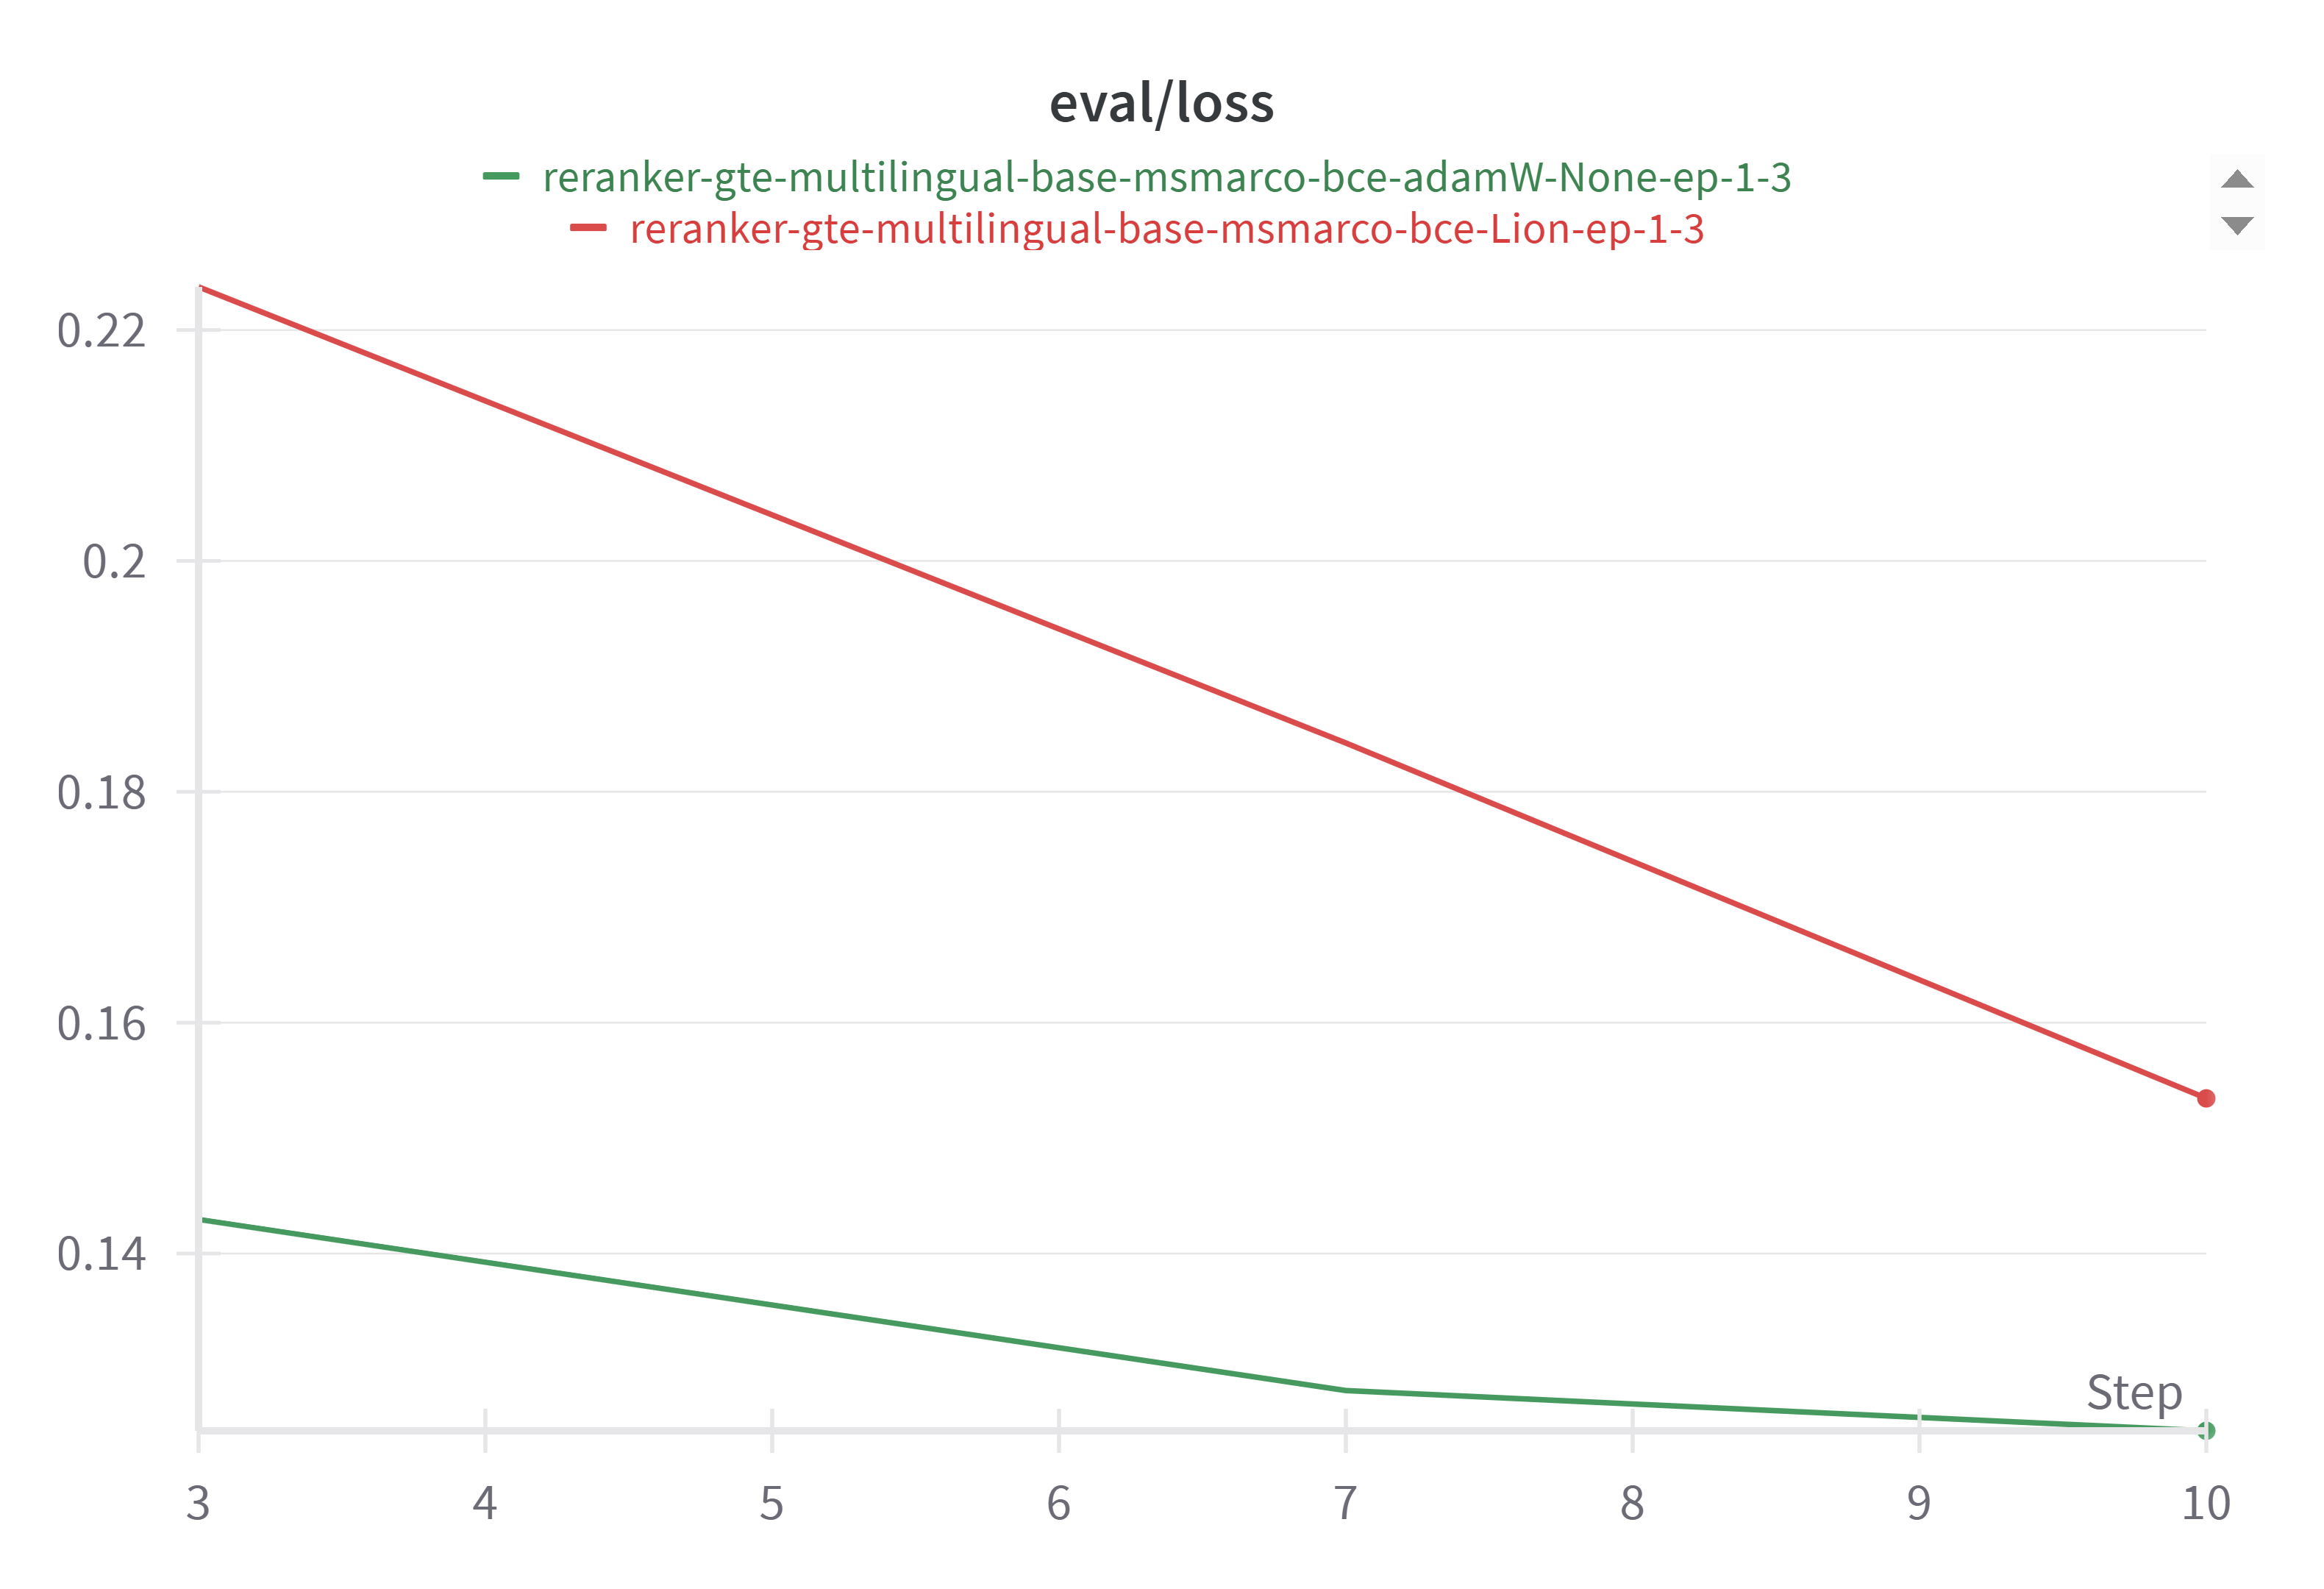
\includegraphics[width=0.8\textwidth]{Figures/gte_adamW_v_lion_eval_loss.png}
    \caption{GTE: Evaluation Loss Comparison}
    \label{fig:gte_eval_loss}
\end{figure}

\begin{figure}[H]
    \centering
    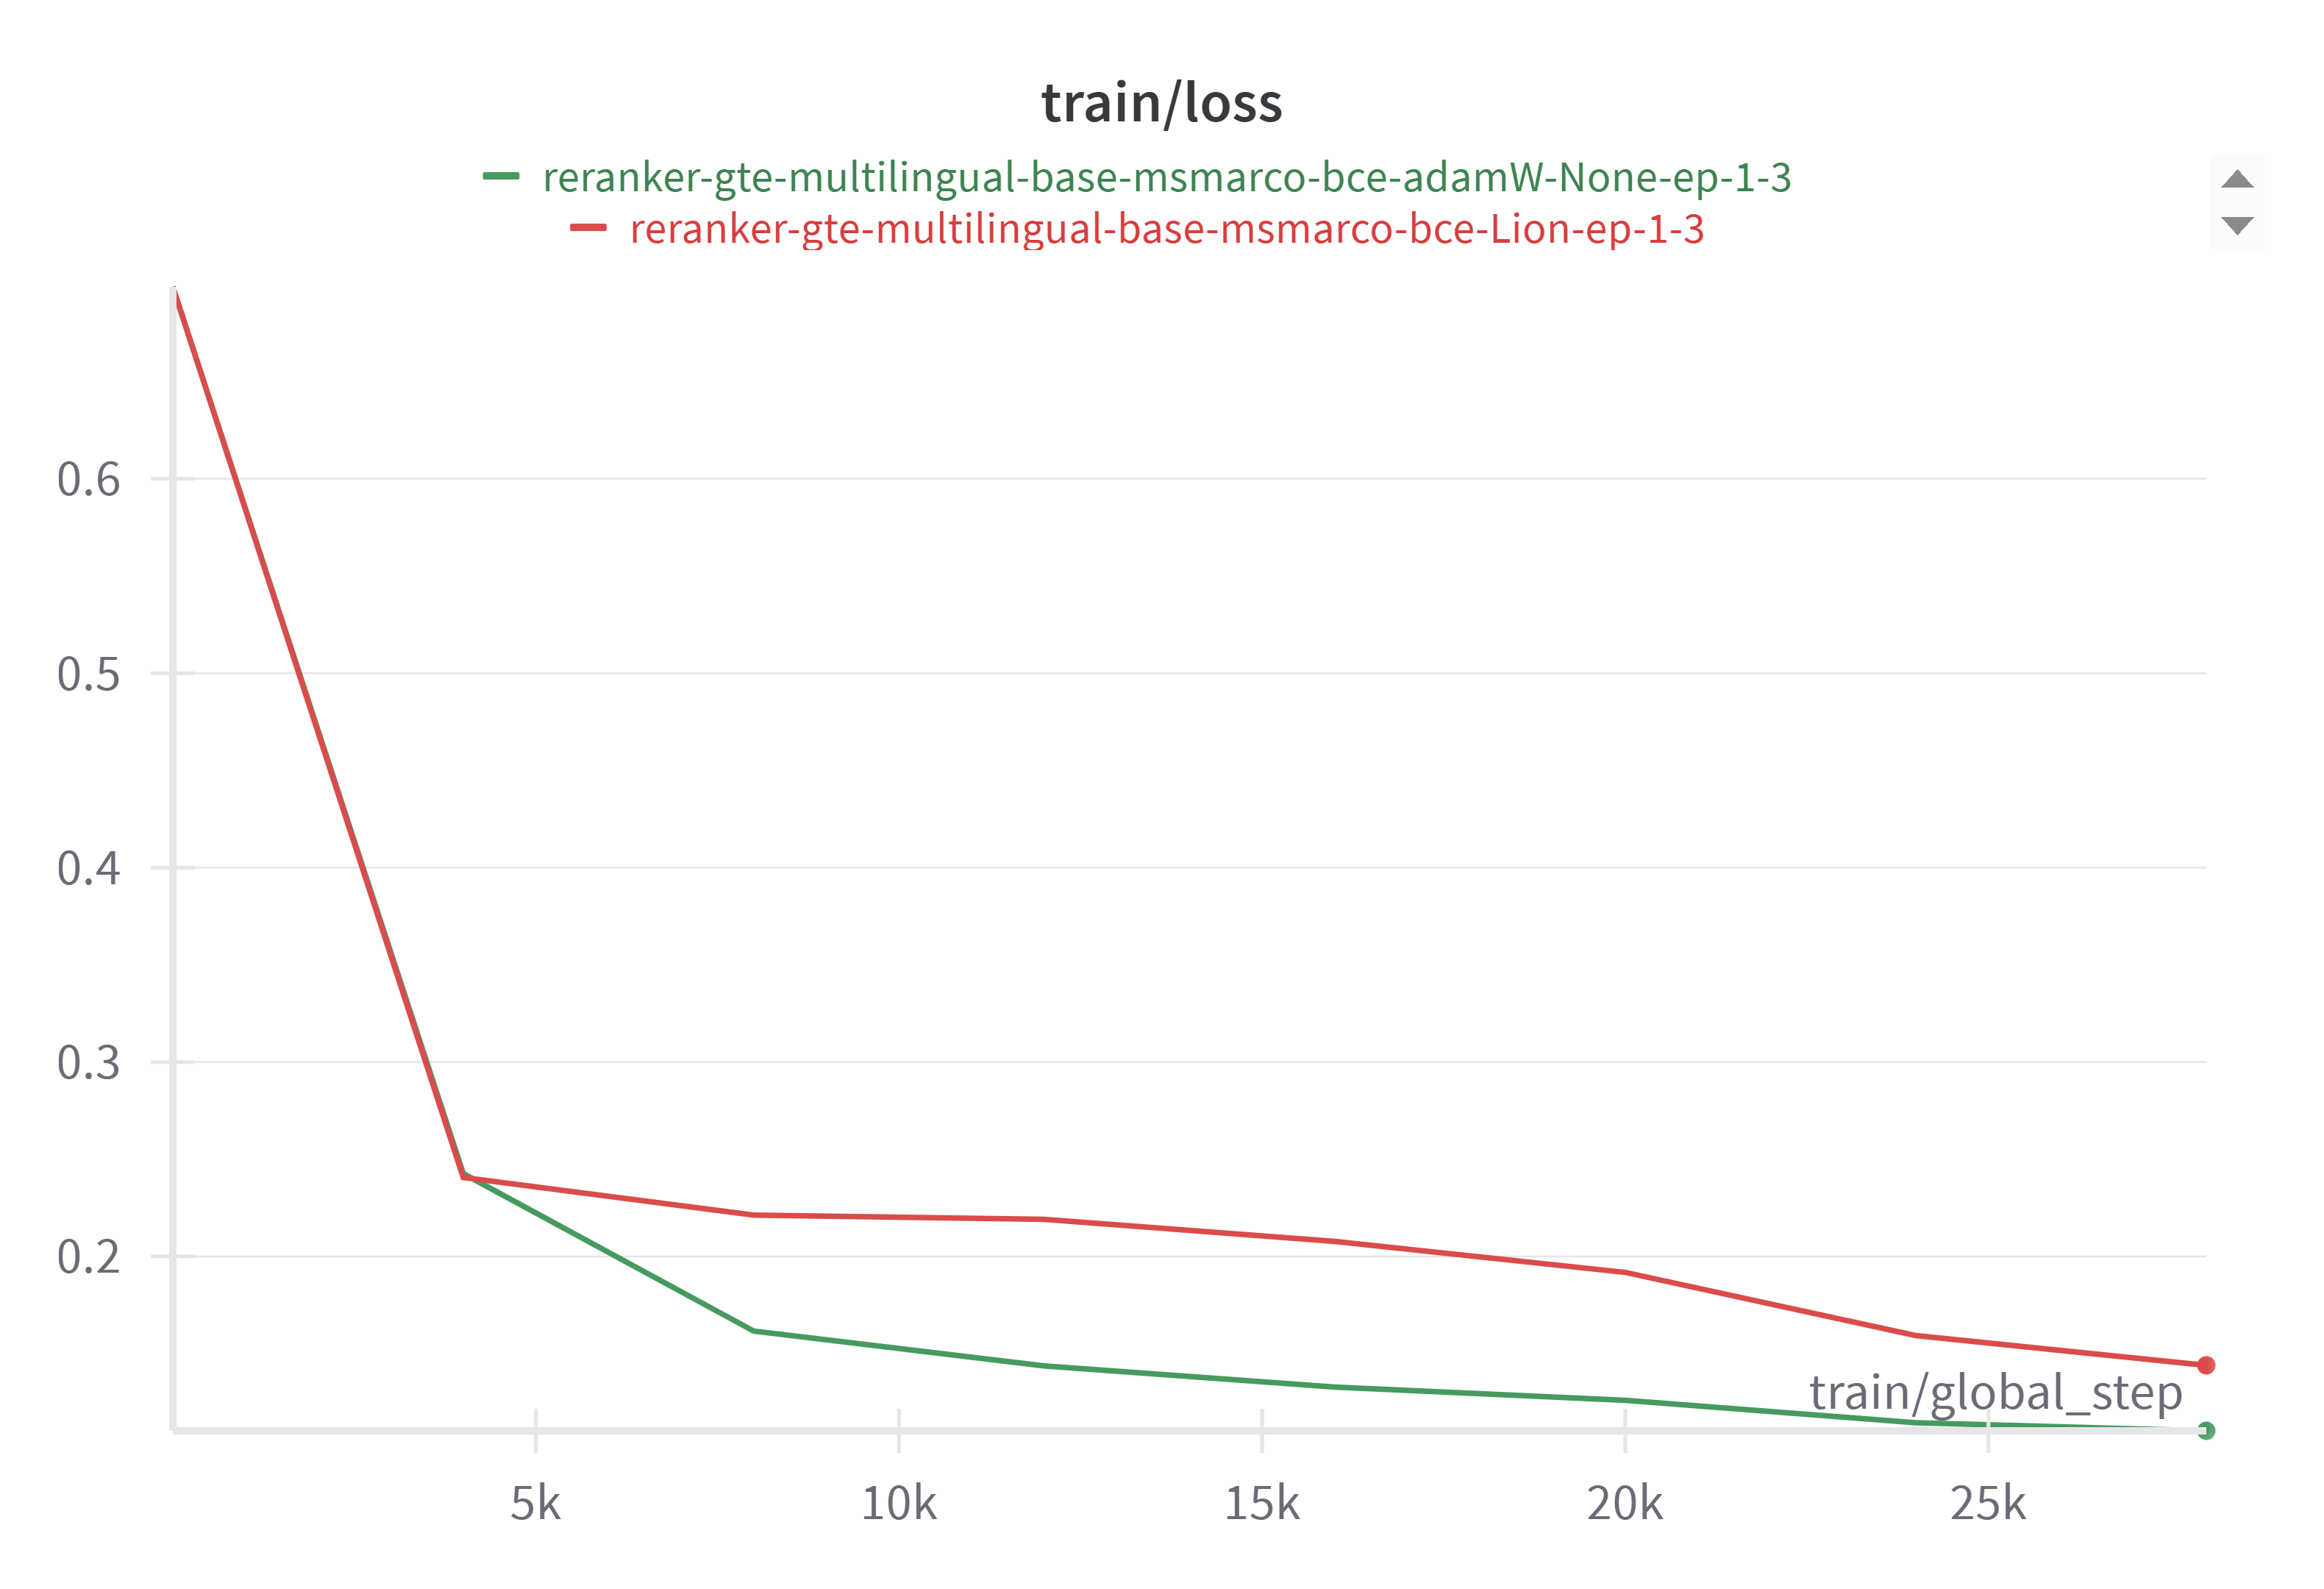
\includegraphics[width=0.8\textwidth]{Figures/gte_adamW_v_lion_train_loss.png}
    \caption{GTE: Training Loss Progression}
    \label{fig:gte_train_loss}
\end{figure}

\begin{figure}[H]
    \centering
    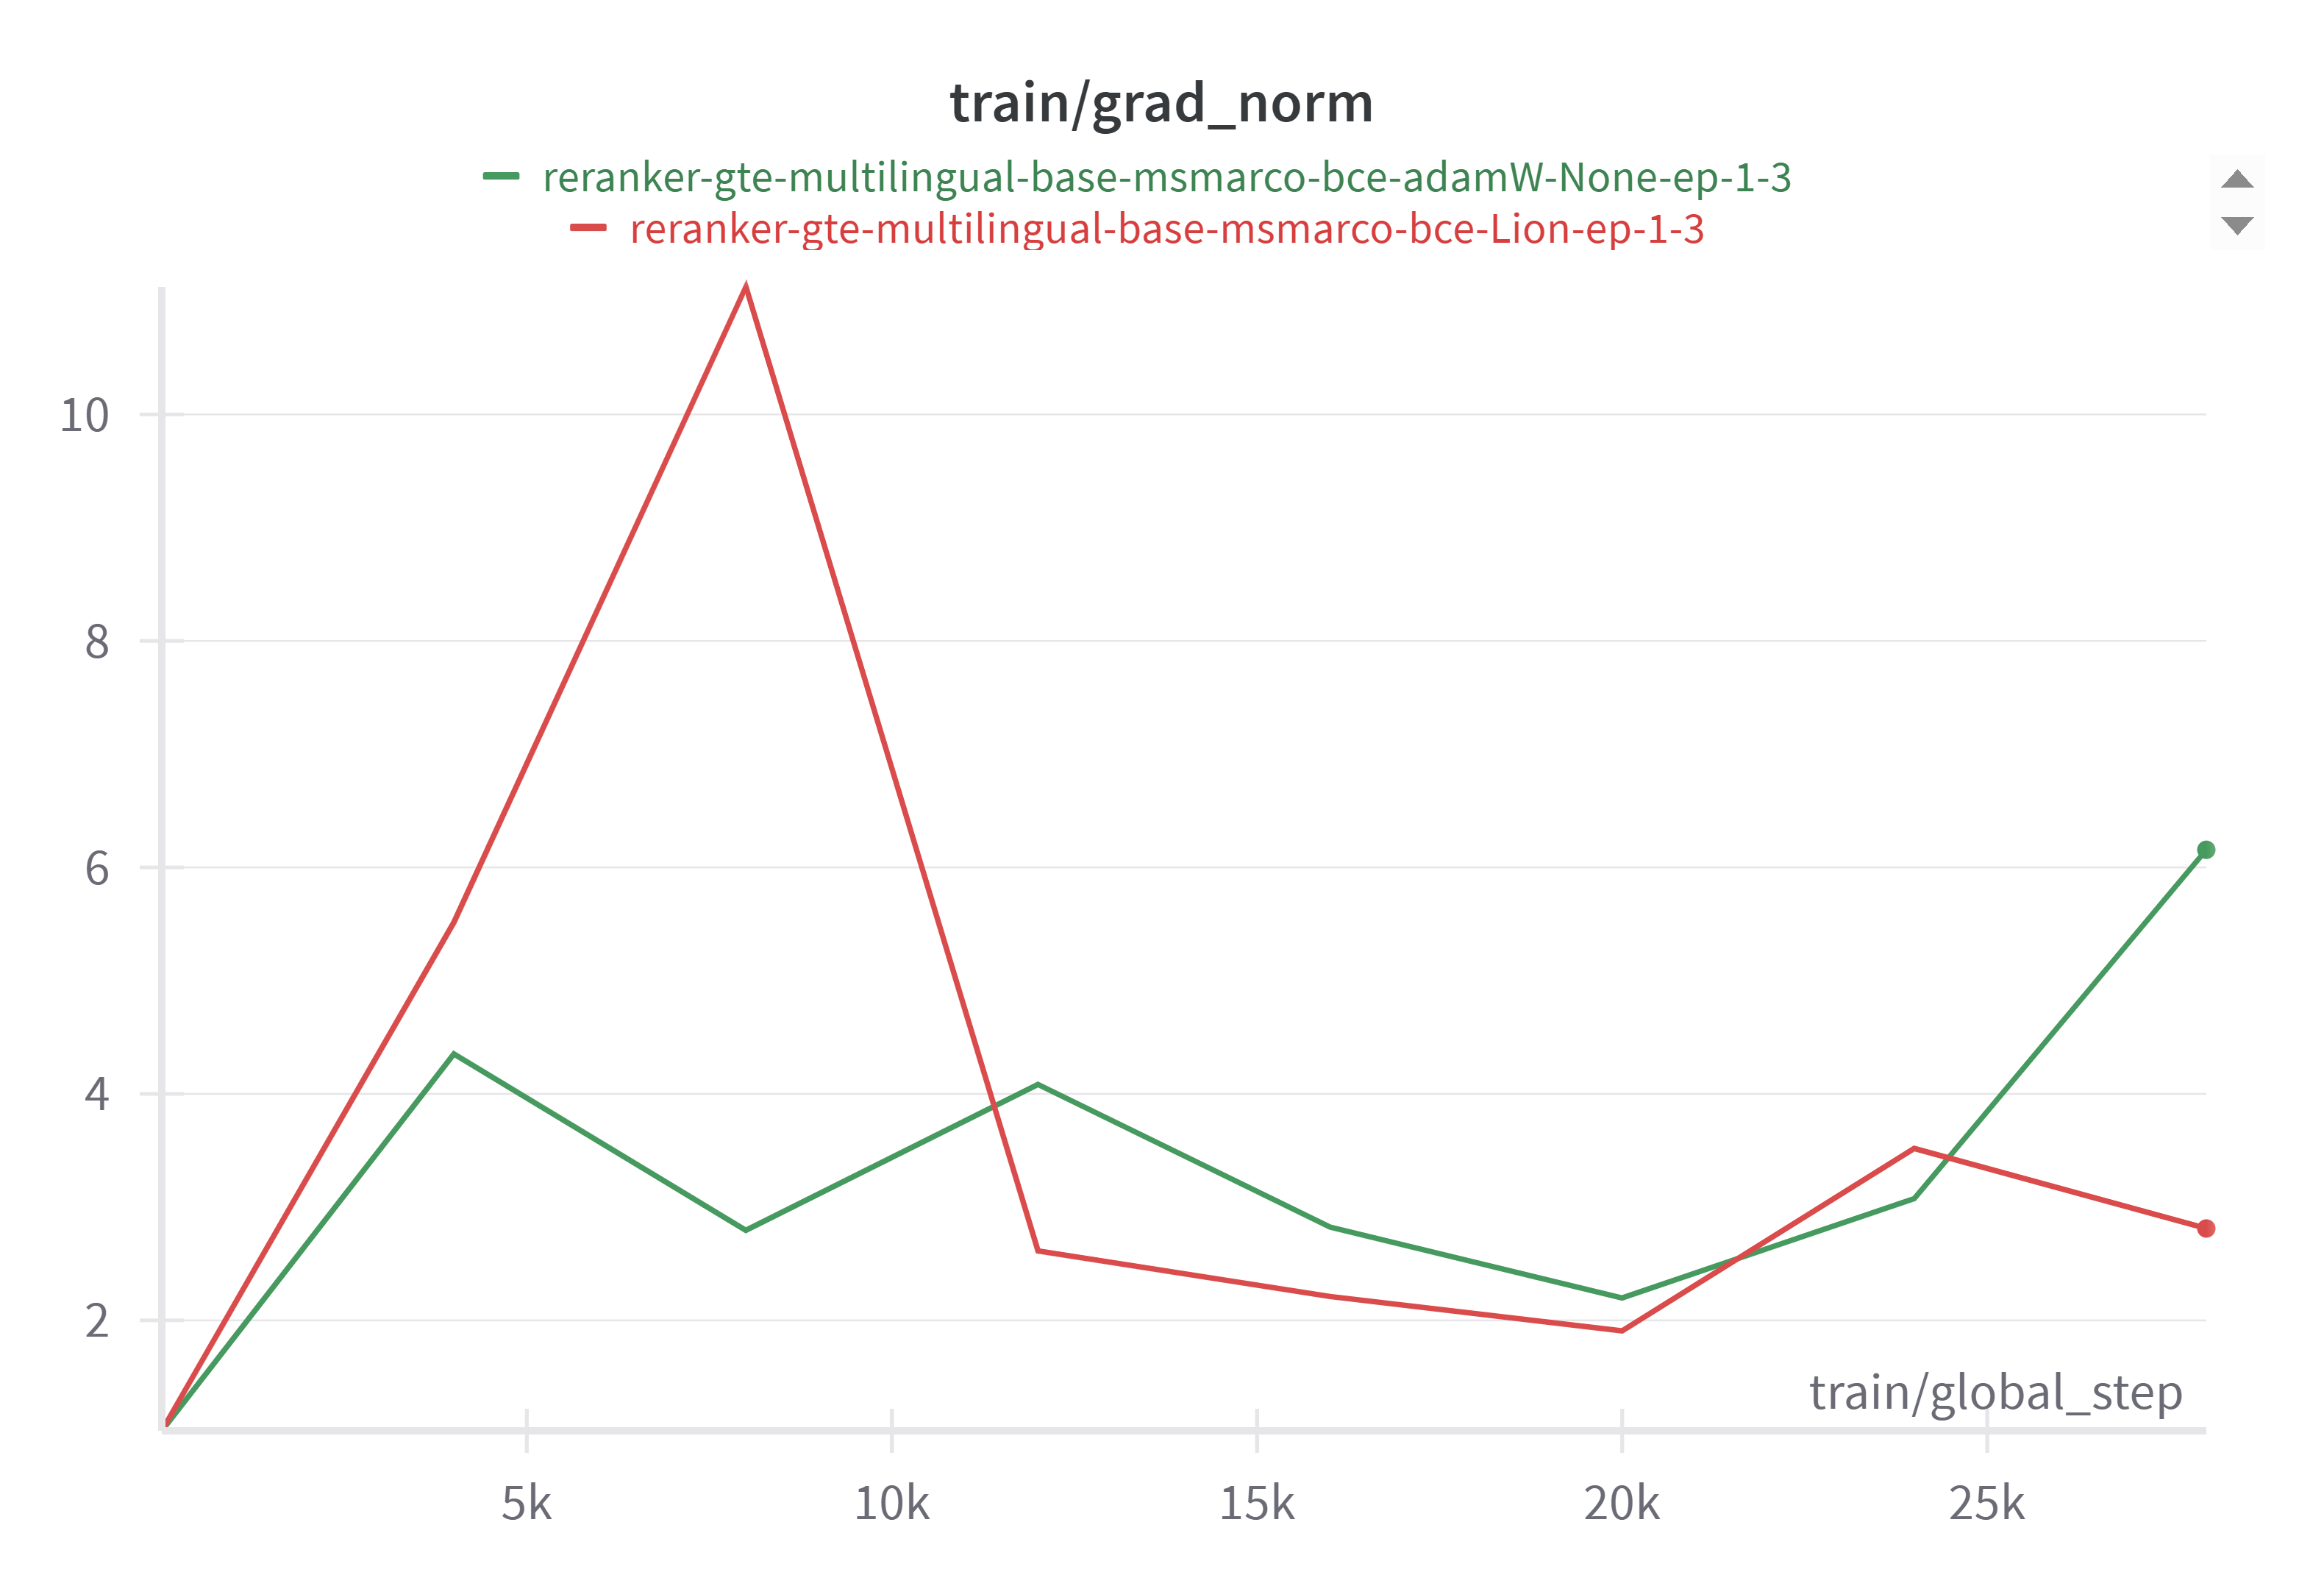
\includegraphics[width=0.8\textwidth]{Figures/gte_adamW_v_lion_grad_norm.png}
    \caption{GTE: Gradient Norm Evolution}
    \label{fig:gte_grad_norm}
\end{figure}

\subsubsection{MiniLM Training Dynamics}

\begin{figure}[H]
    \centering
    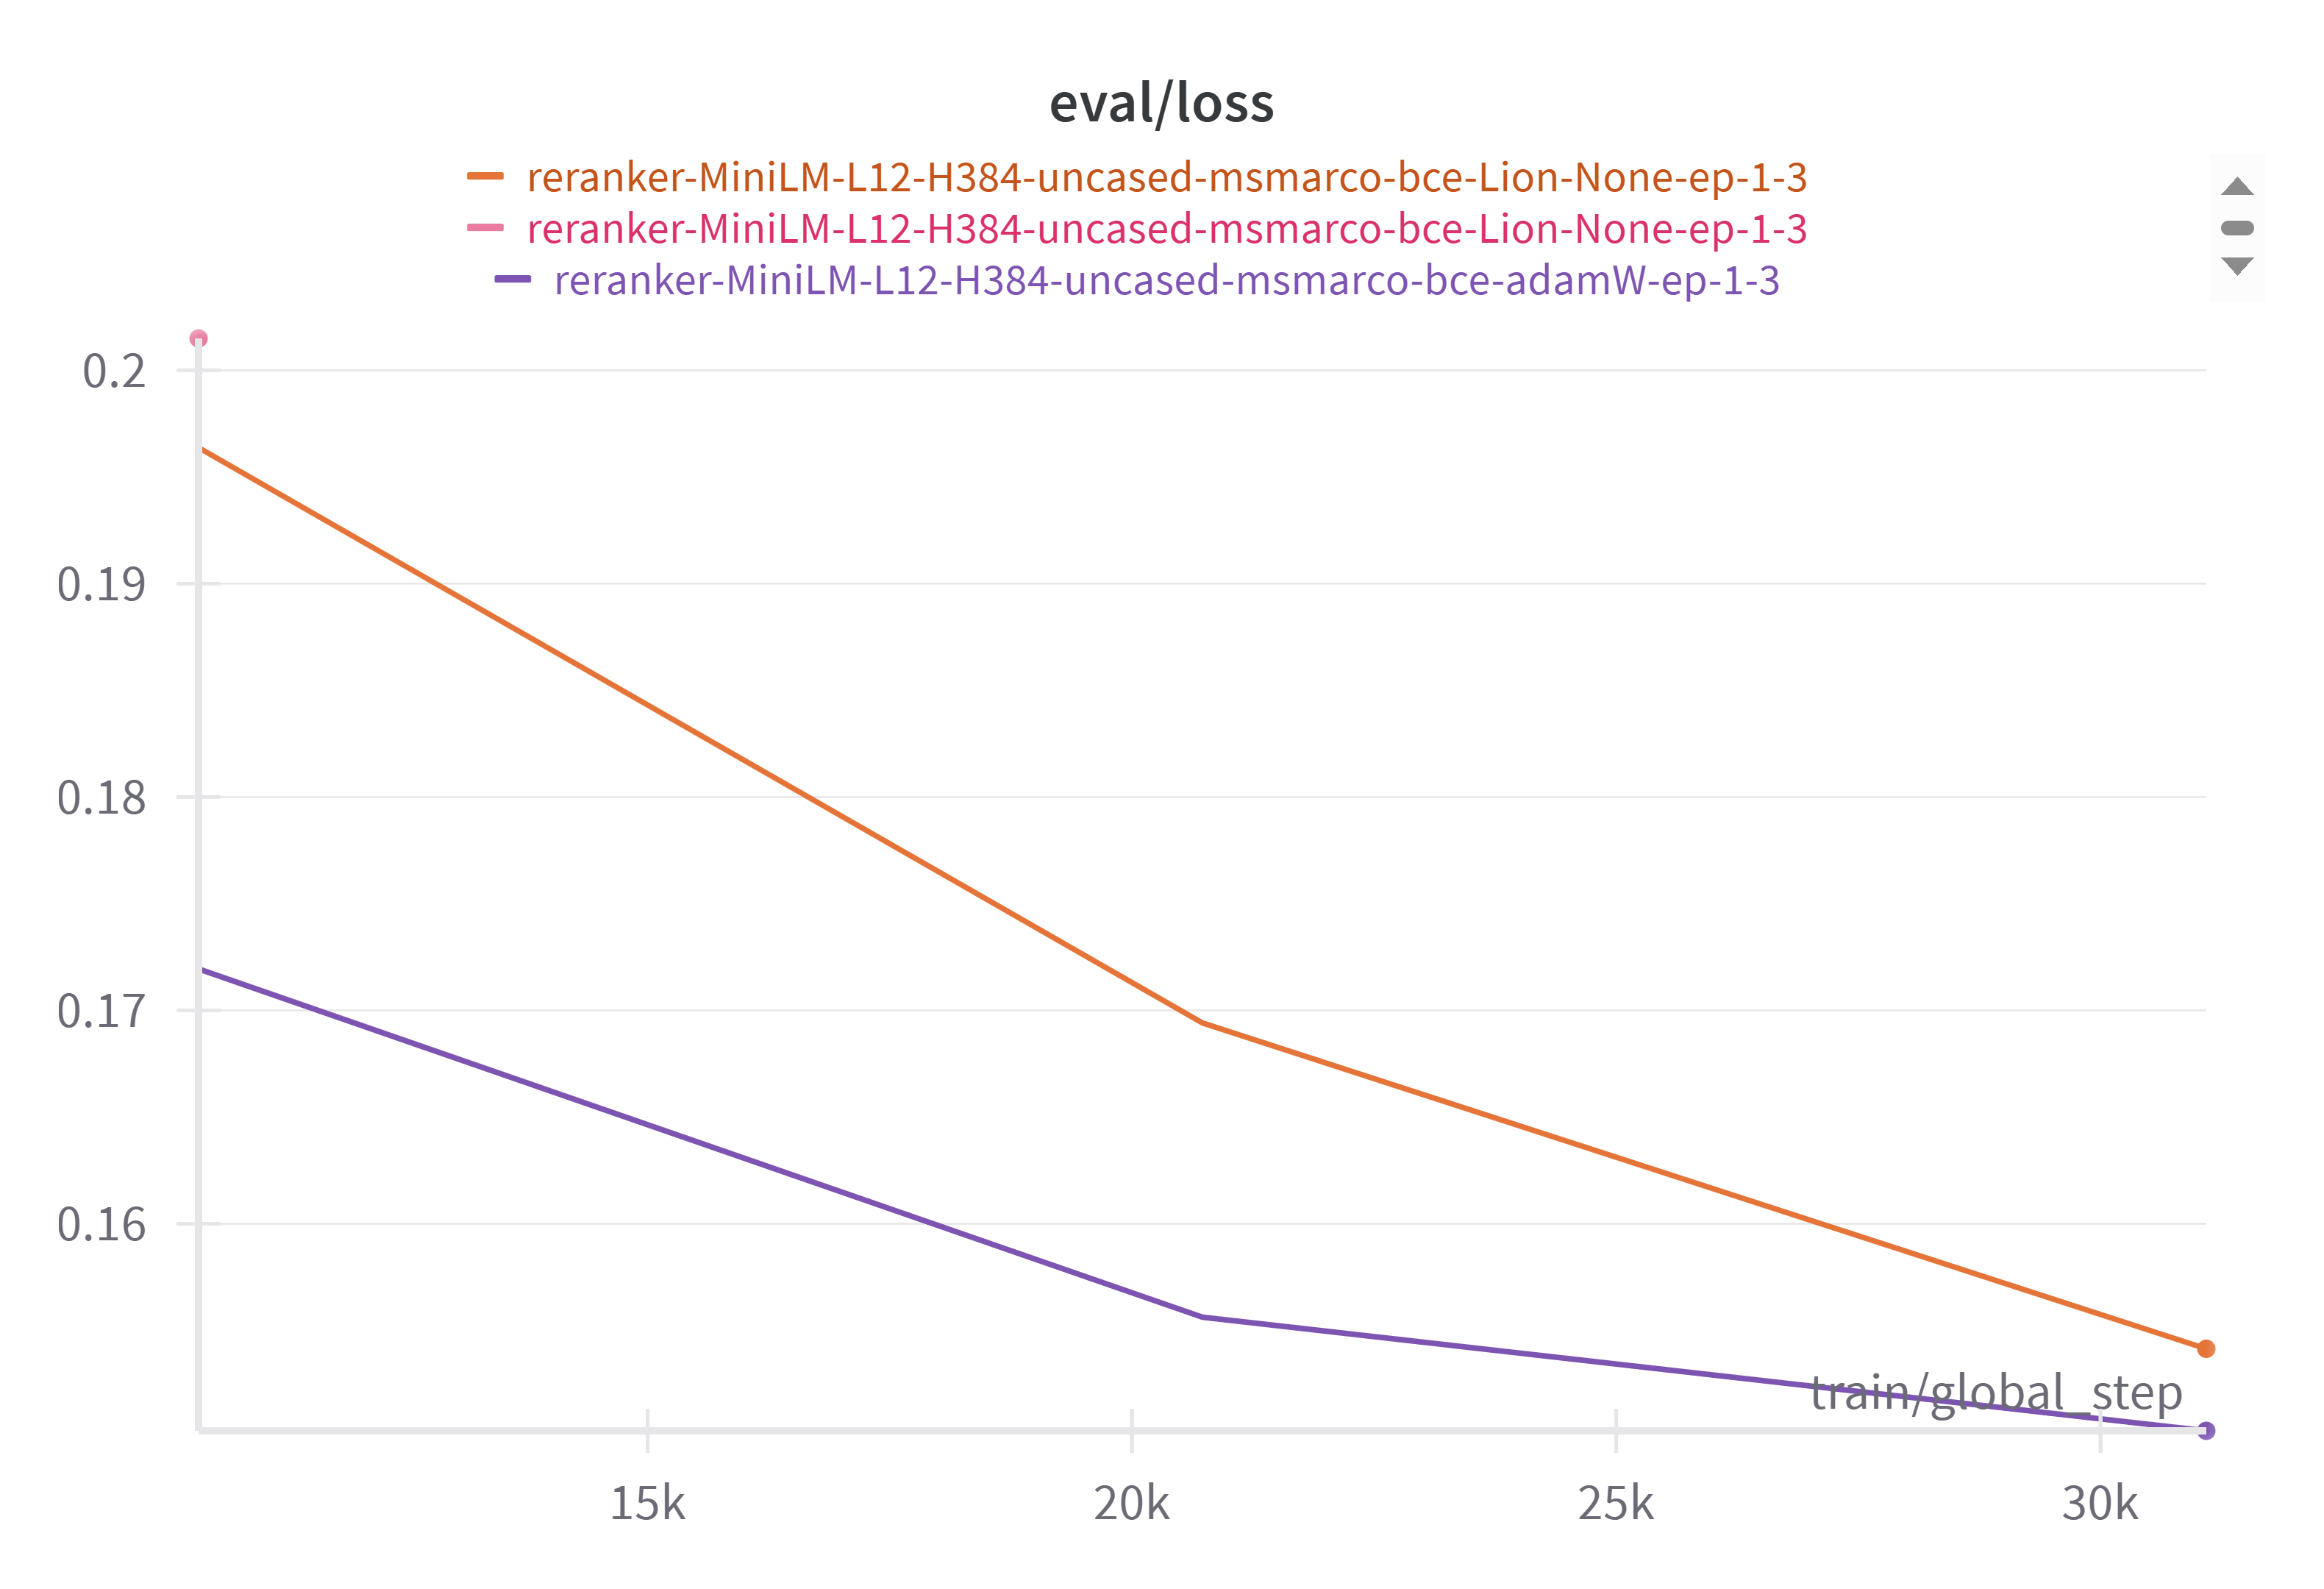
\includegraphics[width=0.8\textwidth]{Figures/microsoft_MiniLM-L12-H384-uncased_adamW_v_Lion_eval_loss.png}
    \caption{MiniLM: Evaluation Loss Comparison}
    \label{fig:minilm_eval_loss}
\end{figure}

\begin{figure}[H]
    \centering
    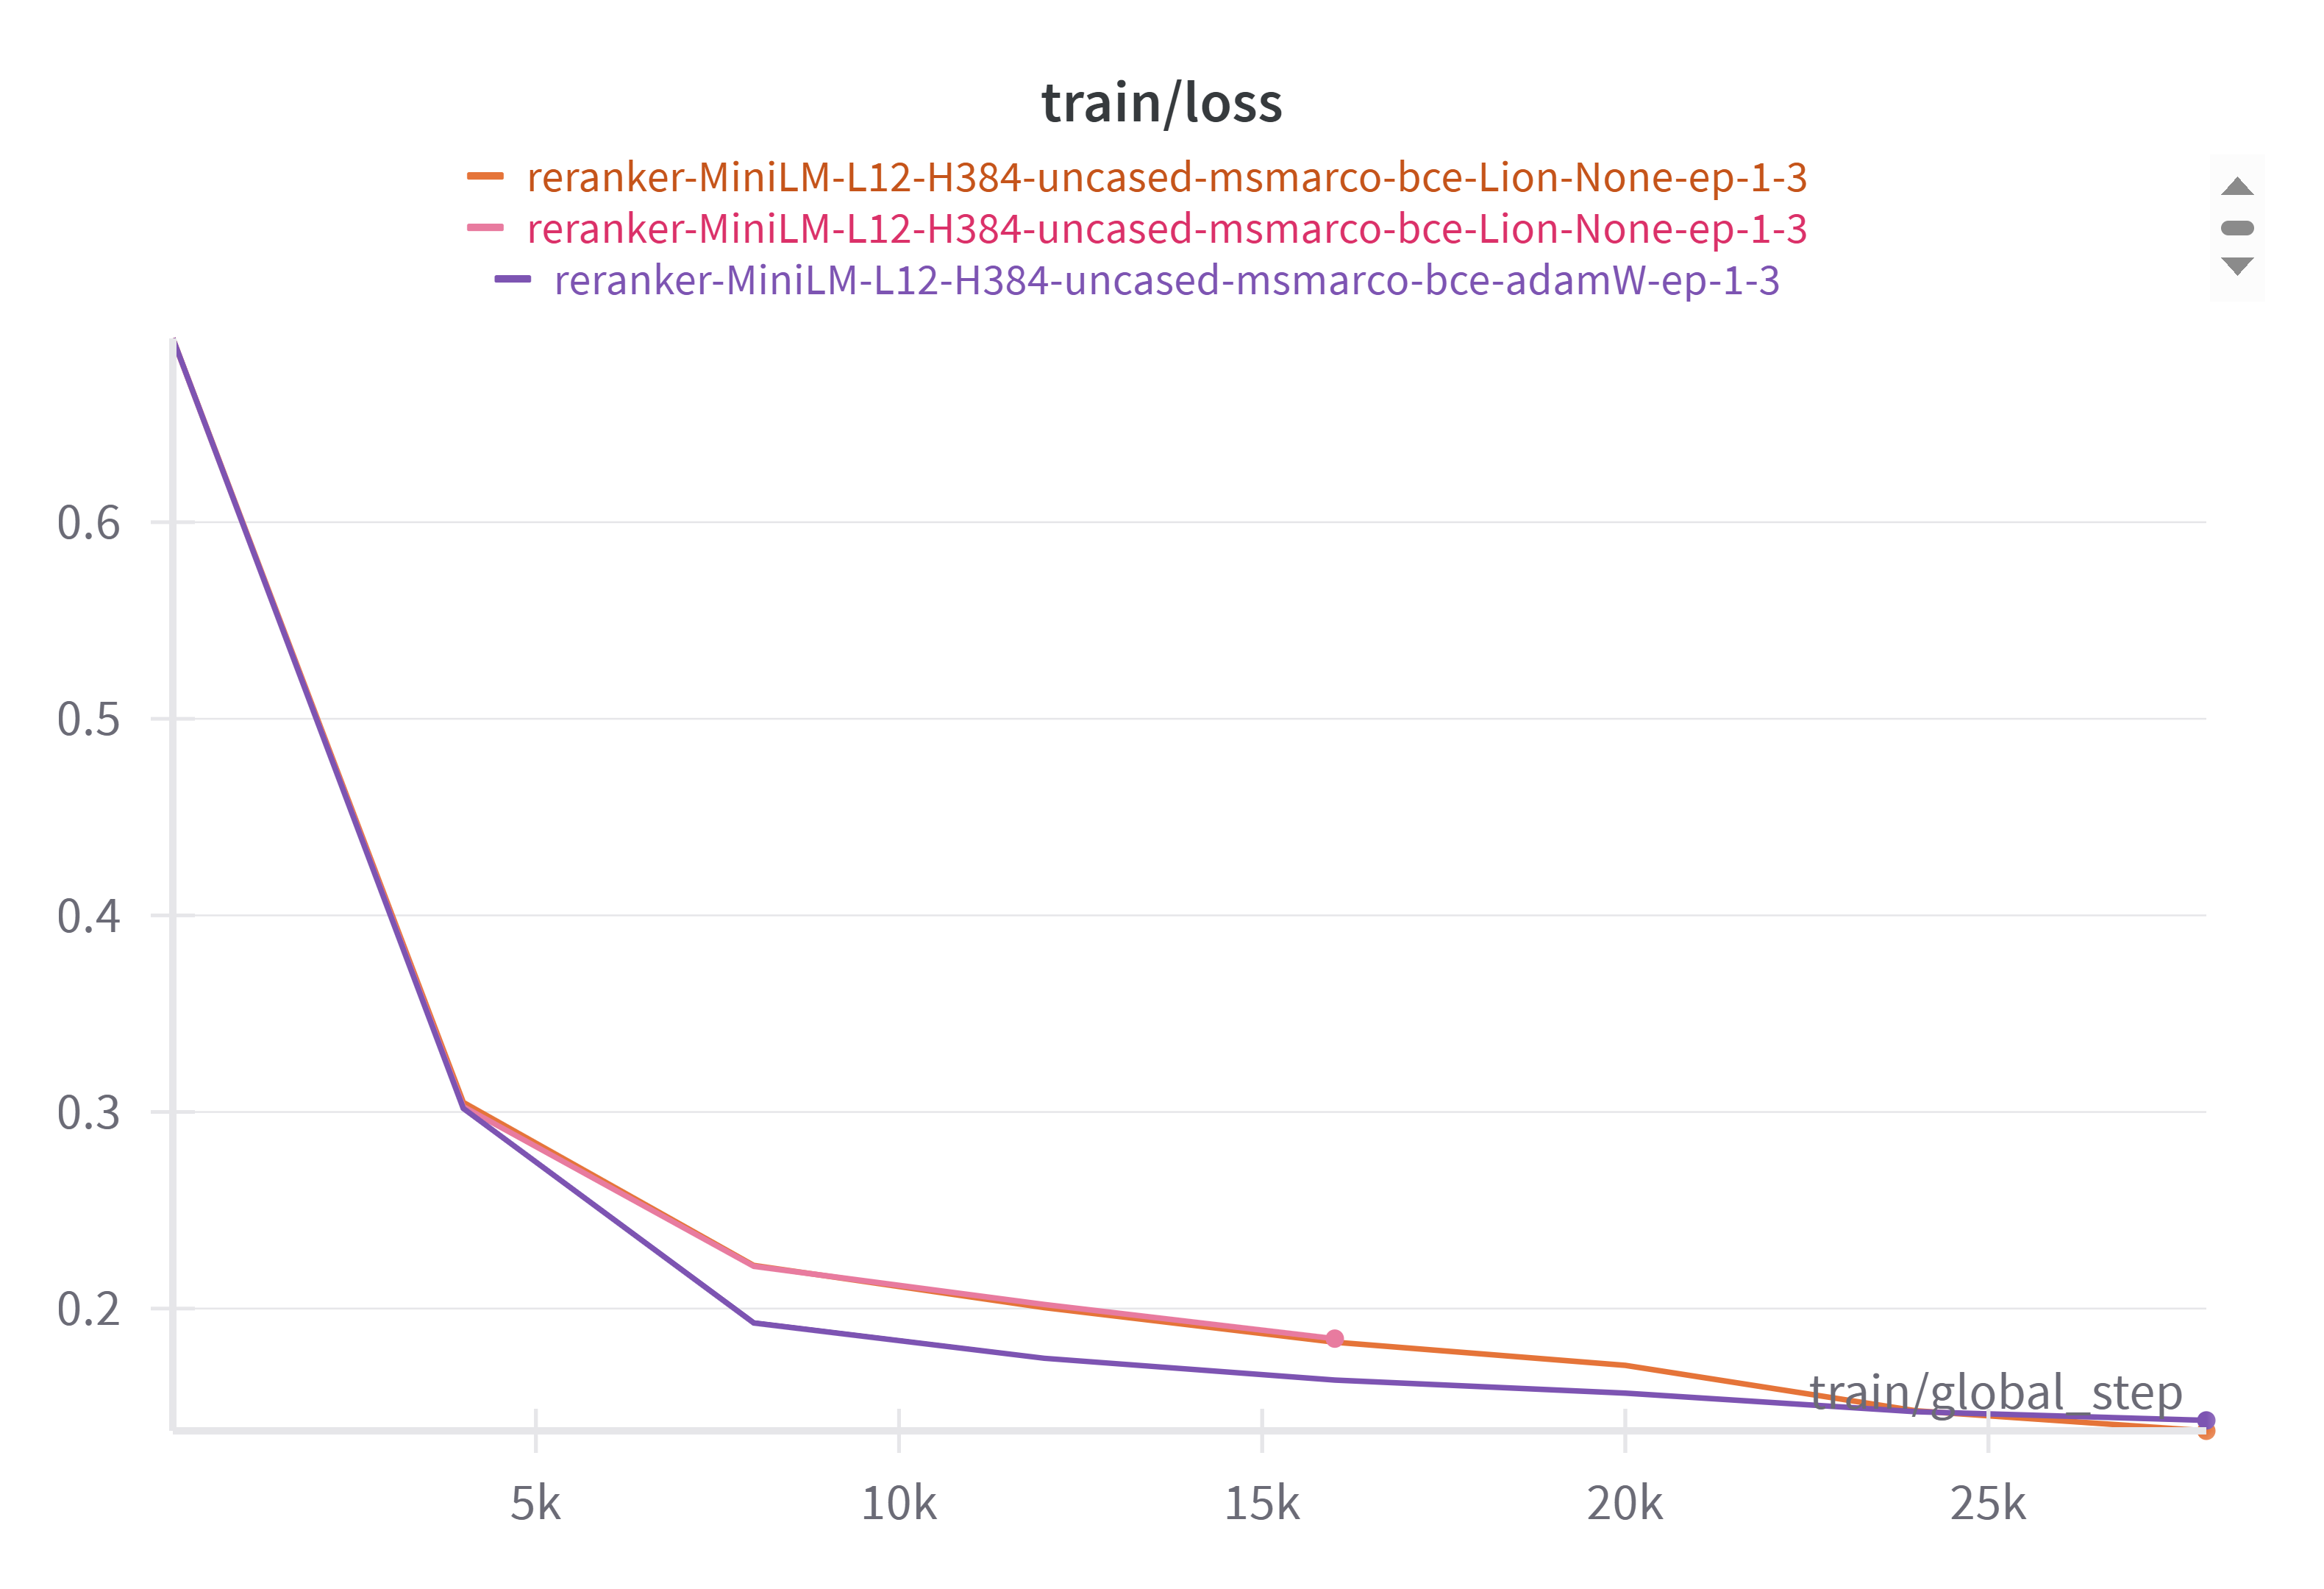
\includegraphics[width=0.8\textwidth]{Figures/microsoft_MiniLM-L12-H384-uncased_adamW_v_Lion_train_loss.png}
    \caption{MiniLM: Training Loss Progression}
    \label{fig:minilm_train_loss}
\end{figure}

\begin{figure}[H]
    \centering
    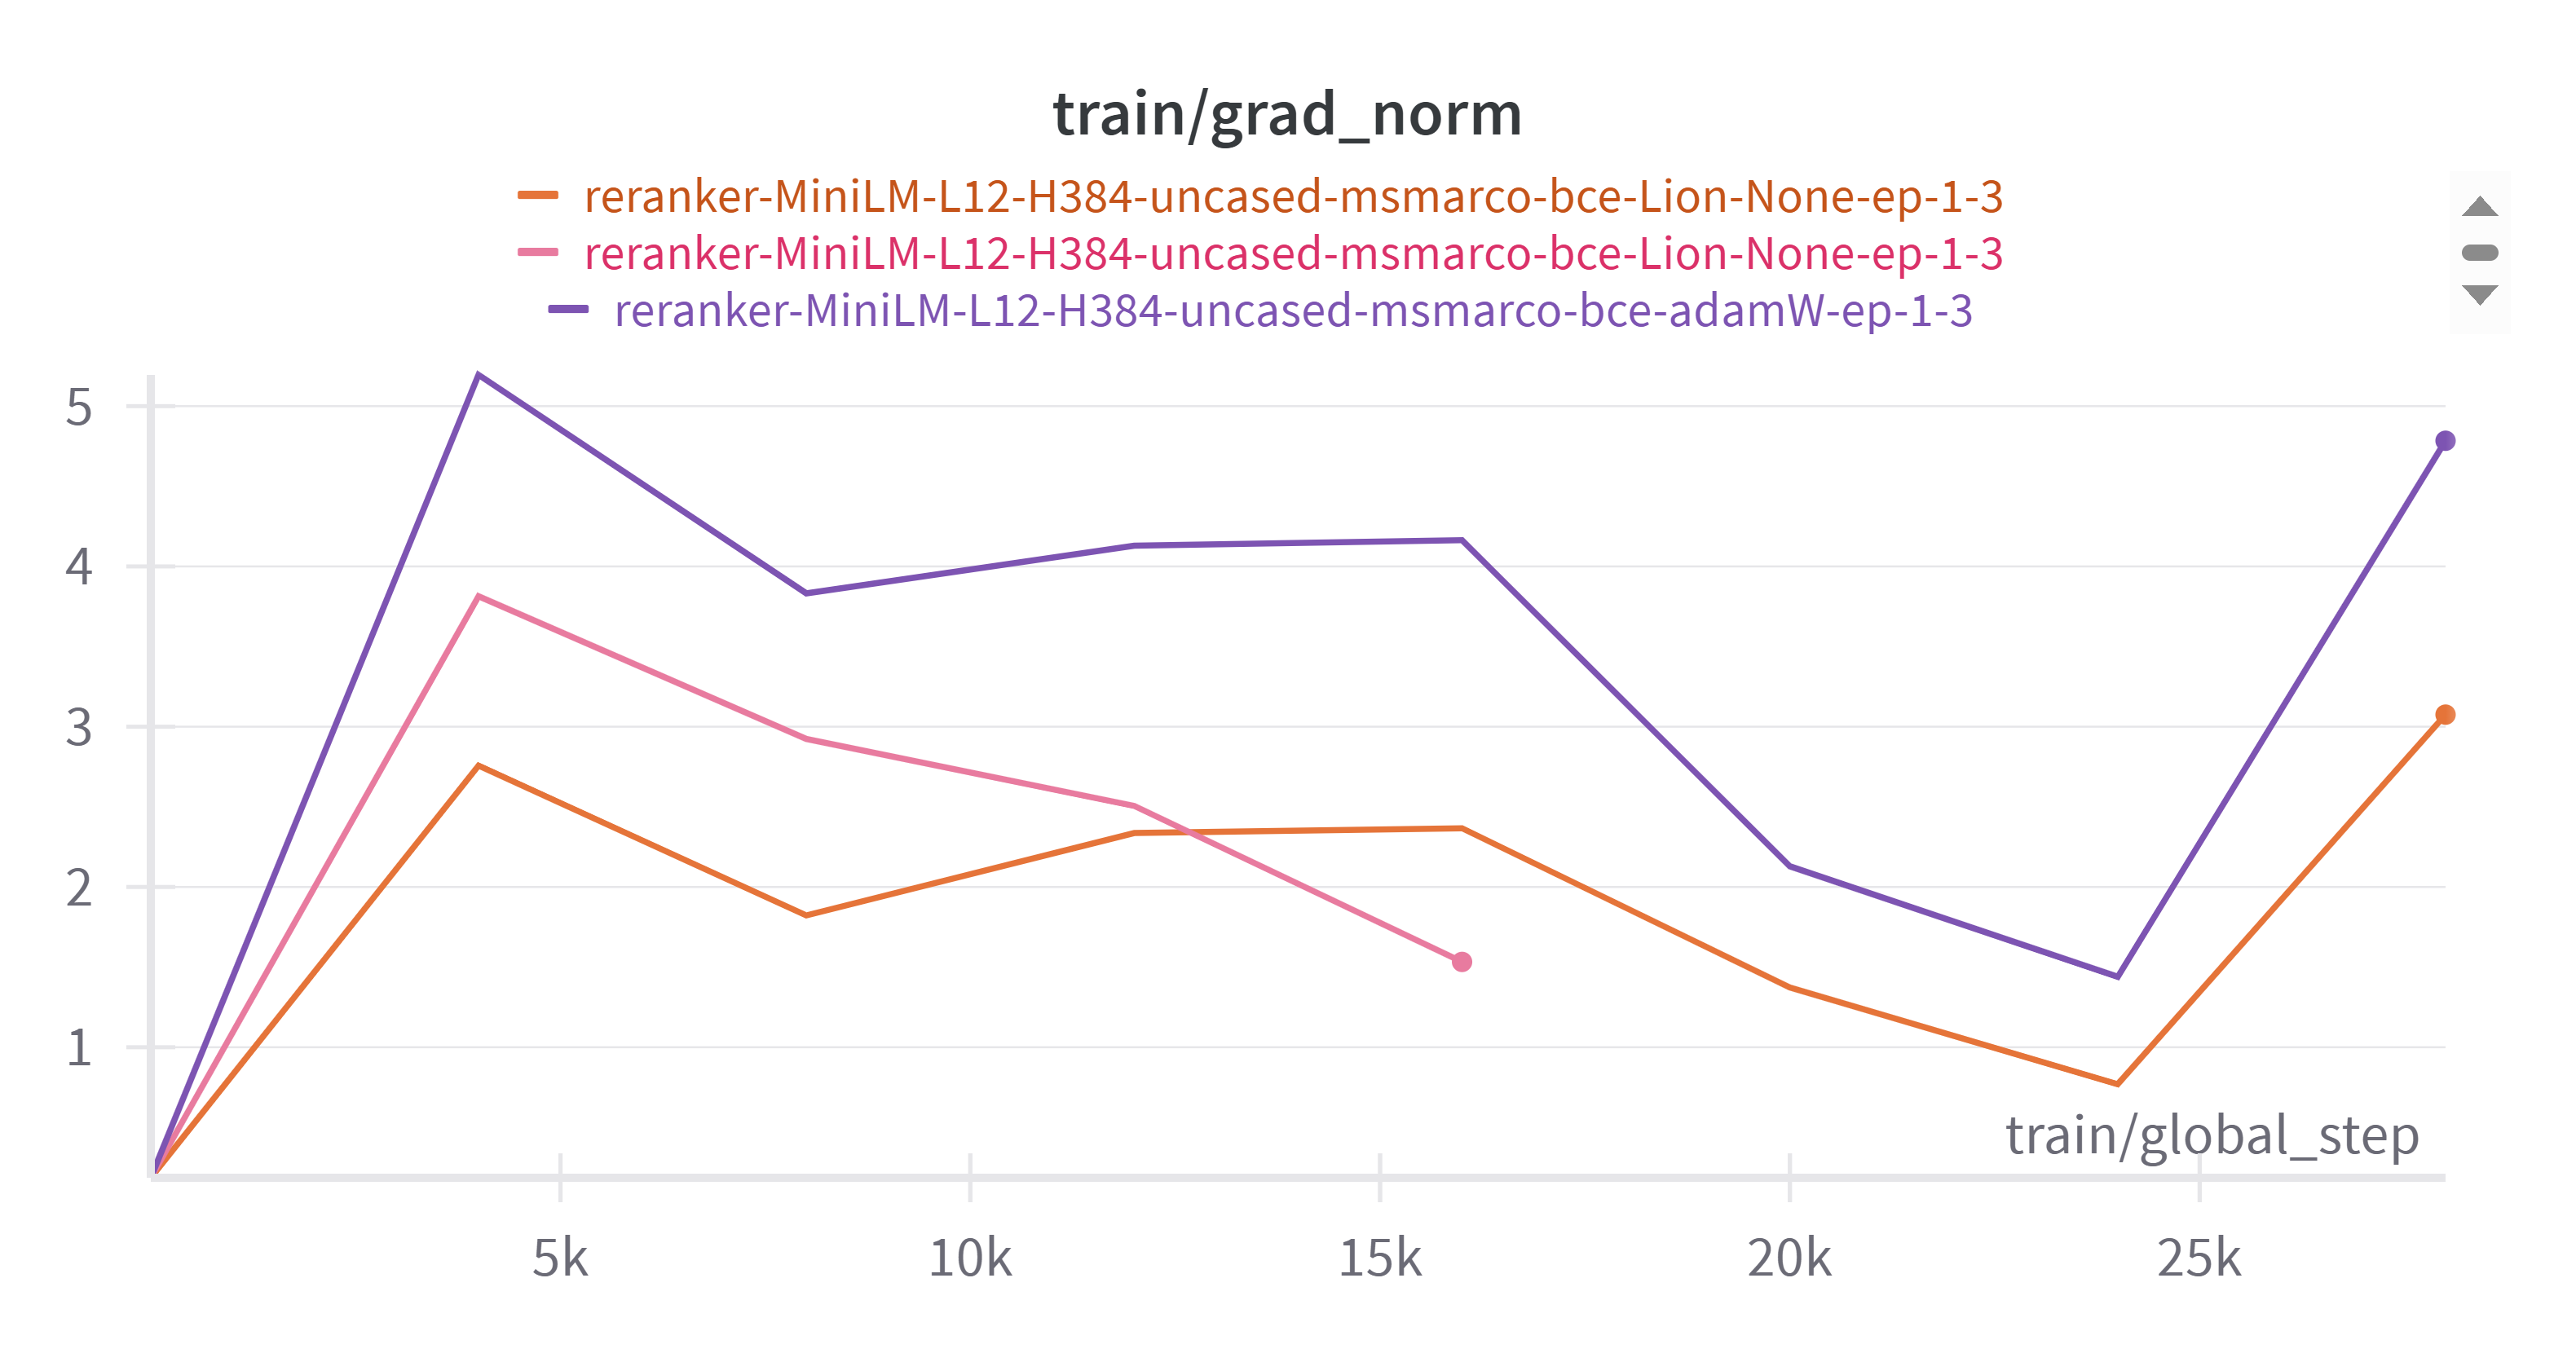
\includegraphics[width=0.8\textwidth]{Figures/microsoft_MiniLM-L12-H384-uncased_adamW_v_Lion_grad_norm.png}
    \caption{MiniLM: Gradient Norm Evolution}
    \label{fig:minilm_grad_norm}
\end{figure}

\section{Discussion of Results}

\subsection{Optimizer Impact Across Models}

The experimental results reveal distinct patterns in how different models interact with the Lion and AdamW optimizers:

\begin{itemize}
    \item \textbf{ModernBERT Performance:} With Lion optimizer and specialized training configuration (lower learning rate of 2e-6 and Cosine Annealing scheduler), ModernBERT achieved the highest overall performance on TREC DL 2019 metrics (NDCG@10: 0.7225, MAP: 0.5115). The training dynamics (Figures \ref{fig:modernbert_eval_loss}-\ref{fig:modernbert_grad_norm}) show more stable convergence with Lion compared to AdamW.
    
    \item \textbf{GTE Behavior:} GTE showed stronger performance with AdamW (NDCG@10: 0.7224) using the standard learning rate (2e-5). The training curves (Figures \ref{fig:gte_eval_loss}-\ref{fig:gte_grad_norm}) indicate that AdamW provided more consistent optimization for this model.
    
    \item \textbf{MiniLM Characteristics:} While MiniLM with AdamW showed better TREC metrics, the Lion optimizer achieved the highest MRR@10 (0.5988) on MS MARCO dev. The training dynamics (Figures \ref{fig:minilm_eval_loss}-\ref{fig:minilm_grad_norm}) suggest that Lion might be particularly effective for certain ranking scenarios.
\end{itemize}

\subsection{Training Dynamics Analysis}

The visualization of training dynamics reveals several key insights:

\begin{itemize}
    \item \textbf{Loss Convergence:} Lion generally shows smoother evaluation loss curves compared to AdamW, particularly evident in the ModernBERT experiments (Figure \ref{fig:modernbert_eval_loss}).
    
    \item \textbf{Gradient Behavior:} The gradient norm plots (Figures \ref{fig:modernbert_grad_norm}, \ref{fig:gte_grad_norm}, \ref{fig:minilm_grad_norm}) show that Lion maintains more consistent gradient magnitudes throughout training.
    
    \item \textbf{Learning Rate Impact:} The Cosine Annealing schedule (Figure \ref{fig:modernbert_lr}) proved particularly effective for ModernBERT with Lion, suggesting that adaptive learning rate strategies can significantly influence optimizer performance.
\end{itemize}

\subsection{Model-Specific Considerations}

The results highlight important model-specific characteristics:

\begin{itemize}
    \item \textbf{Context Length Impact:} Models with longer context capabilities (GTE and ModernBERT, supporting 8192 tokens) generally outperformed MiniLM on TREC DL metrics, suggesting the benefit of extended context for reranking.
    
    \item \textbf{Architecture Influence:} ModernBERT's advanced features (Rotary Positional Embeddings, Flash Attention) appear to synergize well with Lion's optimization approach, particularly with appropriate learning rate scheduling.
    
    \item \textbf{Model Size Considerations:} Despite being smaller, MiniLM showed competitive performance, especially on MRR@10, indicating that model size alone doesn't determine reranking effectiveness.
\end{itemize}


% Chapter Template

\chapter{Summary \& Future Scope of Work}
\label{Chapter6}

This chapter summarizes the key contributions of our research and outlines promising directions for future investigation in optimizer effectiveness for cross-encoder reranking.

\section{Research Summary}

This thesis investigated the comparative effectiveness of Lion and AdamW optimizers for cross-encoder reranking across three transformer architectures: MiniLM, GTE, and ModernBERT.

\subsection{Primary Contributions}

\begin{enumerate}
    \item \textbf{First Systematic Evaluation}: Conducted the first comprehensive comparison of Lion optimizer for cross-encoder information retrieval tasks across multiple architectures.
    
    \item \textbf{Architecture-Optimizer Interaction Analysis}: Demonstrated that optimizer effectiveness varies significantly based on model architecture and training configuration.
    
    \item \textbf{State-of-the-art Results}: Achieved best-in-class performance with ModernBERT + Lion (NDCG@10: 0.7225) and tied best MRR@10 (0.5988) on standard IR benchmarks.
    
    \item \textbf{Training Dynamics Insights}: Provided detailed analysis of convergence patterns and gradient behavior differences between optimizers.
\end{enumerate}

\subsection{Key Findings Summary}

Our experimental results establish that:
\begin{itemize}
    \item \textbf{No Universal Optimizer}: Neither Lion nor AdamW consistently outperforms across all architectures
    \item \textbf{Configuration Sensitivity}: Optimizer effectiveness depends heavily on learning rate and scheduling choices
    \item \textbf{Modern Architecture Benefits}: Advanced transformer features synergize well with Lion's optimization approach
    \item \textbf{Metric-Dependent Performance}: Different optimizers excel on different evaluation metrics
\end{itemize}

\section{Future Scope of Work}

This research opens several promising avenues for future investigation:

\subsection{Immediate Extensions}

\begin{enumerate}
    \item \textbf{Comprehensive Hyperparameter Studies}:
    \begin{itemize}
        \item Systematic grid search for Lion's optimal parameters across model architectures
        \item Investigation of alternative learning rate schedules beyond Cosine Annealing
        \item Analysis of momentum parameter sensitivity
    \end{itemize}

    \item \textbf{Extended Architecture Coverage}:
    \begin{itemize}
        \item Evaluation on larger model sizes (large and extra-large variants)
        \item Testing on emerging transformer architectures (e.g., Mamba, RetNet)
        \item Investigation of decoder-only models for reranking tasks
    \end{itemize}

    \item \textbf{Enhanced Evaluation Scope}:
    \begin{itemize}
        \item Extended evaluation on additional IR benchmarks (BEIR, LoTTE)
        \item Cross-domain evaluation for generalization assessment
        \item Multi-language reranking performance analysis
    \end{itemize}
\end{enumerate}

\subsection{Advanced Research Directions}

\begin{itemize}
    \item \textbf{Theoretical Analysis}: Mathematical characterization of Lion's convergence properties in ranking optimization contexts
    
    \item \textbf{Memory and Efficiency Studies}: Detailed analysis of training time, memory usage, and computational efficiency at scale
    
    \item \textbf{Hybrid Optimization Strategies}: Investigation of combining multiple optimizers during different training phases
    
    \item \textbf{Auto-ML Integration}: Development of automated optimizer selection based on architecture and dataset characteristics
\end{itemize}

\subsection{Practical Applications}

Future work should explore:
\begin{itemize}
    \item \textbf{Production Deployment}: Large-scale evaluation in real-world search systems
    \item \textbf{Specialized Domains}: Medical, legal, and scientific document reranking
    \item \textbf{Multi-Modal Extensions}: Optimization strategies for vision-language retrieval tasks
\end{itemize}

\section{Practical Recommendations}

For practitioners working with cross-encoder reranking:

\begin{itemize}
    \item \textbf{Start with AdamW}: Use AdamW as a robust baseline for initial experiments
    \item \textbf{Consider Lion for Modern Architectures}: Explore Lion optimizer with appropriate learning rate tuning for recent transformer variants
    \item \textbf{Monitor Training Dynamics}: Track multiple metrics and loss curves for optimal checkpoint selection
    \item \textbf{Architecture-Specific Tuning}: Adjust optimizer parameters based on model architecture characteristics
\end{itemize}

\section{Conclusion}

This thesis demonstrates that optimizer choice significantly impacts cross-encoder reranking performance, with the effectiveness varying by architecture and configuration. The Lion optimizer shows particular promise for modern transformer architectures when properly tuned, while AdamW remains a reliable choice across different settings. These findings provide both practical guidance for practitioners and a foundation for future research in neural information retrieval optimization.

\section*{Acknowledgments}

We gratefully acknowledge Modal Labs for providing the cloud computing infrastructure and GPU resources (NVIDIA A100-80GB) that enabled this comprehensive experimental study. 
\end{spacing}

\addcontentsline{toc}{section}{\textbf{References}}
\nocite{*}
\printbibliography
% %	BIBLIOGRAPHY
% %----------------------------------------------------------------------------------------

% %----------------------------------------------------------------------------------------
\end{sloppypar}
\end{document}  
